% LaTeX support: latex@mdpi.com 
% In case you need support, please attach all files that are necessary for compiling as well as the log file, and specify the details of your LaTeX setup (which operating system and LaTeX version / tools you are using).

%=================================================================
\documentclass[geosciences,article,submit,moreauthors,pdftex]{Definitions/mdpi} 
% \usepackage{graphics}
\usepackage{amsthm, amssymb, amsfonts}
\usepackage{array,longtable}
\usepackage{overpic}
\graphicspath{{./Images/}}
% If you would like to post an early version of this manuscript as a preprint, you may use preprint as the journal and change 'submit' to 'accept'. The document class line would be, e.g., \documentclass[preprints,article,accept,moreauthors,pdftex]{mdpi}. This is especially recommended for submission to arXiv, where line numbers should be removed before posting. For preprints.org, the editorial staff will make this change immediately prior to posting.

%--------------------
% Class Options:
%--------------------
%----------
% journal
%----------
% Choose between the following MDPI journals:
% acoustics, actuators, addictions, admsci, aerospace, agriculture, agriengineering, agronomy, algorithms, animals, antibiotics, antibodies, antioxidants, applsci, arts, asc, asi, atmosphere, atoms, axioms, batteries, bdcc, behavsci, beverages, bioengineering, biology, biomedicines, biomimetics, biomolecules, biosensors, brainsci, buildings, cancers, carbon, catalysts, cells, ceramics, challenges, chemengineering, chemistry, chemosensors, children, cleantechnol, climate, clockssleep, cmd, coatings, colloids, computation, computers, condensedmatter, cosmetics, cryptography, crystals, dairy, data, dentistry, designs, diagnostics, diseases, diversity, drones, econometrics, economies, education, ejihpe, electrochem, electronics, energies, entropy, environments, epigenomes, est, fermentation, fibers, fire, fishes, fluids, foods, forecasting, forests, fractalfract, futureinternet, futurephys, galaxies, games, gastrointestdisord, gels, genealogy, genes, geohazards, geosciences, geriatrics, hazardousmatters, healthcare, heritage, highthroughput, horticulturae, humanities, hydrology, ijerph, ijfs, ijgi, ijms, ijns, ijtpp, informatics, information, infrastructures, inorganics, insects, instruments, inventions, iot, j, jcdd, jcm, jcp, jcs, jdb, jfb, jfmk, jimaging, jintelligence, jlpea, jmmp, jmse, jnt, jof, joitmc, jpm, jrfm, jsan, land, languages, laws, life, literature, logistics, lubricants, machines, magnetochemistry, make, marinedrugs, materials, mathematics, mca, medicina, medicines, medsci, membranes, metabolites, metals, microarrays, micromachines, microorganisms, minerals, modelling, molbank, molecules, mps, mti, nanomaterials, ncrna, neuroglia, nitrogen, notspecified, nutrients, ohbm, optics, particles, pathogens, pharmaceuticals, pharmaceutics, pharmacy, philosophies, photonics, physics, plants, plasma, polymers, polysaccharides, preprints, proceedings, processes, proteomes, psych, publications, quantumrep, quaternary, qubs, reactions, recycling, religions, remotesensing, reports, resources, risks, robotics, safety, sci, scipharm, sensors, separations, sexes, signals, sinusitis, smartcities, sna, societies, socsci, soilsystems, sports, standards, stats, surfaces, surgeries, sustainability, symmetry, systems, technologies, test, toxics, toxins, tropicalmed, universe, urbansci, vaccines, vehicles, vetsci, vibration, viruses, vision, water, wem, wevj

%---------
% article
%---------
% The default type of manuscript is "article", but can be replaced by: 
% abstract, addendum, article, benchmark, book, bookreview, briefreport, casereport, changes, comment, commentary, communication, conceptpaper, conferenceproceedings, correction, conferencereport, expressionofconcern, extendedabstract, meetingreport, creative, datadescriptor, discussion, editorial, essay, erratum, hypothesis, interestingimages, letter, meetingreport, newbookreceived, obituary, opinion, projectreport, reply, retraction, review, perspective, protocol, shortnote, supfile, technicalnote, viewpoint
% supfile = supplementary materials

%----------
% submit
%----------
% The class option "submit" will be changed to "accept" by the Editorial Office when the paper is accepted. This will only make changes to the frontpage (e.g., the logo of the journal will get visible), the headings, and the copyright information. Also, line numbering will be removed. Journal info and pagination for accepted papers will also be assigned by the Editorial Office.

%------------------
% moreauthors
%------------------
% If there is only one author the class option oneauthor should be used. Otherwise use the class option moreauthors.

%---------
% pdftex
%---------
% The option pdftex is for use with pdfLaTeX. If eps figures are used, remove the option pdftex and use LaTeX and dvi2pdf.

%=================================================================
\firstpage{1} 
\makeatletter 
\setcounter{page}{\@firstpage} 
\makeatother
\pubvolume{xx}
\issuenum{1}
\articlenumber{5}
\pubyear{2019}
\copyrightyear{2019}
%\externaleditor{Academic Editor: name}
\history{Received: date; Accepted: date; Published: date}
%\updates{yes} % If there is an update available, un-comment this line

%% MDPI internal command: uncomment if new journal that already uses continuous page numbers 
%\continuouspages{yes}

%------------------------------------------------------------------
% The following line should be uncommented if the LaTeX file is uploaded to arXiv.org
%\pdfoutput=1

%=================================================================
% Add packages and commands here. The following packages are loaded in our class file: fontenc, calc, indentfirst, fancyhdr, graphicx, lastpage, ifthen, lineno, float, amsmath, setspace, enumitem, mathpazo, booktabs, titlesec, etoolbox, amsthm, hyphenat, natbib, hyperref, footmisc, geometry, caption, url, mdframed, tabto, soul, multirow, microtype, tikz

% \PassOptionsToPackage[OT1]{fontenc} % options for packages loaded elsewhere
%=================================================================
%% Please use the following mathematics environments: Theorem, Lemma, Corollary, Proposition, Characterization, Property, Problem, Example, ExamplesandDefinitions, Hypothesis, Remark, Definition, Notation, Assumption
%% For proofs, please use the proof environment (the amsthm package is loaded by the MDPI class).

%=================================================================
% Full title of the paper (Capitalized)
\Title{Revealing trends in geophysics using text analysis}

% Author Orchid ID: enter ID or remove command
\newcommand{\orcidauthorA}{0000-0002-7928-5736} % Add \orcidA{} behind the author's name
\newcommand{\orcidauthorB}{0000-0002-9743-7107} % Add \orcidB{} behind the author's name
\newcommand{\orcidauthorC}{0000-0002-9389-7579} % Add \orcidB{} behind the author's name

% Authors, for the paper (add full first names)
\Author{Timofey Eltsov $^{1,\dagger}$\orcidA{}, Maxim Yutkin $^{2}$\orcidB{}, Tadeusz W. Patzek $^{3}$\orcidC{}} % and Firstname Lastname $^{2,}$*}

% Authors, for metadata in PDF
\AuthorNames{Timofey Eltsov and Tadeusz W. Patzek}

% Affiliations / Addresses (Add [1] after \address if there is only one affiliation.)
\address{$^{1}$ \quad Ali I. Al-Naimi Petroleum Engineering Research Center, King Abdullah University of Science and Technology; timofey.eltsov@kaust.edu.sa\\
$^{2}$ \quad Ali I. Al-Naimi Petroleum Engineering Research Center, King Abdullah University of Science and Technology; maxim.yutkin@kaust.edu.sa\\
$^{3}$ \quad Ali I. Al-Naimi Petroleum Engineering Research Center, King Abdullah University of Science and Technology; tadeusz.patzek@kaust.edu.sa}

% Contact information of the corresponding author
\corres{Correspondence: timofey.eltsov@kaust.edu.sa; Tel.: +966128087182}

% Current address and/or shared authorship
\firstnote{Current address: 4700 KAUST, Thuwal, 23955-6900, Saudi Arabia}
% The commands \thirdnote{} till \eighthnote{} are available for further notes

%\simplesumm{} % Simple summary

%\conference{} % An extended version of a conference paper

% Abstract (Do not insert blank lines, i.e. \\) 
\abstract{Professional language evolution reveals the advances in geophysics: researchers enthusiastically describe new methods of survey, data processing techniques, and objects of their study. Geophysicists publish their cutting-edge research at international conferences proceedings to share their achievements with the world. Tracking changes in the language allows one to identify trends and the current state of the science. Here, we describe the text analysis of the last 38 Annual Conferences organized by the Society of Exploration Geophysicists, one of the biggest geophysical gatherings. We split 24,500 articles into words and phrases and analyze the change in their usage frequency over time. We find that in 2019 the phrase ``neural network'' is used more often than ``field data.'' The word ``shale'' has become less commonly used, but the term ``unconventional'' is growing in occurrence. An analysis of conference materials and metadata allows one to identify trends in a specific field of knowledge and predict the development in the near future.}

% Keywords
\keyword{geophysics; web data analysis; data mining; data analysis; text mining; words analysis;}

% The fields PACS, MSC, and JEL may be left empty or commented out if not applicable
%\PACS{J0101}
%\MSC{}
%\JEL{}

%%%%%%%%%%%%%%%%%%%%%%%%%%%%%%%%%%%%%%%%%%
% Only for the journal Diversity
%\LSID{\url{http://}}

%%%%%%%%%%%%%%%%%%%%%%%%%%%%%%%%%%%%%%%%%%
% Only for the journal Applied Sciences:
%\featuredapplication{Authors are encouraged to provide a concise description of the specific application or a potential application of the work. This section is not mandatory.}
%%%%%%%%%%%%%%%%%%%%%%%%%%%%%%%%%%%%%%%%%%

%%%%%%%%%%%%%%%%%%%%%%%%%%%%%%%%%%%%%%%%%%
% Only for the journal Data:
%\dataset{DOI number or link to the deposited data set in cases where the data set is published or set to be published separately. If the data set is submitted and will be published as a supplement to this paper in the journal Data, this field will be filled by the editors of the journal. In this case, please make sure to submit the data set as a supplement when entering your manuscript into our manuscript editorial system.}

%\datasetlicense{license under which the data set is made available (CC0, CC-BY, CC-BY-SA, CC-BY-NC, etc.)}

%%%%%%%%%%%%%%%%%%%%%%%%%%%%%%%%%%%%%%%%%%
% Only for the journal Toxins
%\keycontribution{The breakthroughs or highlights of the manuscript. Authors can write one or two sentences to describe the most important part of the paper.}

%\setcounter{secnumdepth}{4}
%%%%%%%%%%%%%%%%%%%%%%%%%%%%%%%%%%%%%%%%%%
\begin{document}
%%%%%%%%%%%%%%%%%%%%%%%%%%%%%%%%%%%%%%%%%%

%%%%%%%%%%%%%%%%%%%%%%%%%%%%%%%%%%%%%%%%%%
% \setcounter{section}{-1} %% Remove this when starting to work on the template.
%\section{How to Use this Template}
%The template details the sections that can be used in a manuscript. Note that the order and names of article sections may differ from the requirements of the journal (e.g., the positioning of the Materials and Methods section). Please check the instructions for authors page of the journal to verify the correct order and names. For any questions, please contact the editorial office of the journal or support@mdpi.com. For LaTeX related questions please contact latex@mdpi.com.
%%The order of the section titles is: Introduction, Materials and Methods, Results, Discussion, Conclusions for these journals: aerospace,algorithms,antibodies,antioxidants,atmosphere,axioms,biomedicines,carbon,crystals,designs,diagnostics,environments,fermentation,fluids,forests,fractalfract,informatics,information,inventions,jfmk,jrfm,lubricants,neonatalscreening,neuroglia,particles,pharmaceutics,polymers,processes,technologies,viruses,vision

\section{Introduction}
The last four decades saw a tremendous change in geophysics. An increase in computing power and technological progress allowed geophysicists to solve more and more complicated tasks. At the same time, the field of application of geophysics is expanding; the market of geophysical services is changing. We assume that a change in geophysical tasks, applications, geography, and technology will inevitably lead to a shift in the professional language. If one can track changes in the frequency of terms used in recent years, one can shed light on the current state of the industry and possibly predict future changes. Authors apply language processing methods to analyze changes in the professional language in geophysics.

The biases of different origin complicate big data \citep{Glauner2018}. In machine learning, the difference between training data set and test data set can cause biases. Massive sample study can lead to bias associated with an error resulting from sampling or study design \citep{Kaplan2014}. Supposedly, it is better to have a smaller and more representative data set rather than a much bigger but biased data. We want to understand what the modern geophysical language looks like and what the future of geophysics will be. In this paper, we analyze only scientific articles presented at the Society of Exploration Geophysicists (SEG) Annual Conference and Exhibition. The committee selects the papers for the conference each year; this is the initial filtering. Also, it is worth noting that presenting at such a meeting is a demonstration of the technical capabilities of industrial companies and the scientific viability of academic institutions. Each annual conference proceedings are a cross-section of the state of geophysics, and we use it for analysis and predictions.

The SEG Annual Conference and Exhibition is one of the biggest gatherings of geophysicists in the world. Abstracts of the SEG Annual Conferences are a representation of the state of geophysical science, devoted mainly to the oil and gas industry. Articles in the electronic version for the 38 years are available for analysis \citep{SEG}. The SEG conducts all their Annual conferences in the USA, and the last one was held in San Antonio, TX. For analysis, the authors selected the proceedings of the SEG Annual Conference, as the most representative set, that reflects state-of-art technologies in geophysics. Each conference proceedings is a reflection of the state of the industry in a particular year since, at this event, both academic institutions and the industry present their best achievements in the field.

Besides conference proceedings, one can use journal articles for data mining as the volume of the data for one year is comparable to the SEG Annual Conference and Exhibition Proceedings. The number of publications per year is smaller, but they consist of full-size papers. However, the release of articles in journals is carried out periodically, e.g., monthly or quarterly; at the conference, this happens once a year. The research materials are usually published in journals and reported at conferences; the proceedings include many of the results from full-sized articles. Moreover, the number of research teams presenting their work is several times larger in the case of analysis of conference materials compared to the study of one particular journal. SEG Annual Conference proceedings represent a collection of scientific research from a large number of scientific teams in one place for each of the 38 years. This approach allows one to conduct a unique study and trace the dynamics of changes in the industry.

%%%%%%%%%%%%%%%%%%%%%%%%%%%%%%%%%%%%%%%%%%%
\section{Materials and Methods}

We use open-source Python libraries: to transform, filter and process the text: TextBlob, NLTK (Natural Language Toolkit), argparse, Pandas, Scrapy, Requests-HTML, sqlite3, and NumPy. For printing the graphs, we use Matplotlib, Plotly, PIL (Python Imaging Library), and others.

We used digital versions of the SEG Annual Conference proceedings that have been available online for 38 years. Fig. \ref{scheme_workflow} shows the workflow scheme. Abstracts from the 1980s consisted of 1 or 2 pages; in the 1990s, it increased to four pages per abstract. We digitized articles in PDF format from the SEG digital library website, converted them into plain TXT format using ``pdftotext'' with ``nopgbrk'' (ignore page breaks), ``enc ASCII7'' (sets ASCII7 encoding for the output) and ``eol'' (sets the end-of-line convention) flags. The text damp was filtered to remove common words, misspellings, \textit{etc.} from a NLTK dictionary, ``stopwords.'' After the initial filtering, we tokenized the text by year and obtained si-, bi-, and trigrams\footnote{``sigram'' - a word, ``bigram'' - two-word phrase, ``trigram'' - three-word phrase}. Further, we counted the number of times each word or phrase was repeated. Finally, the entire text for 38 years is a three-dimensional array of words and phrases with the corresponding number of repetitions for each year. We then analyze the list of words and phrases during observation time and display the results in a graphical format.

While digitalizing abstracts from the 1980s, recognition errors, merged words, and typos occur. Therefore, we present the results of phrase count only for the period from 1990 to 2019.

\begin{figure}[ht!]
\centering
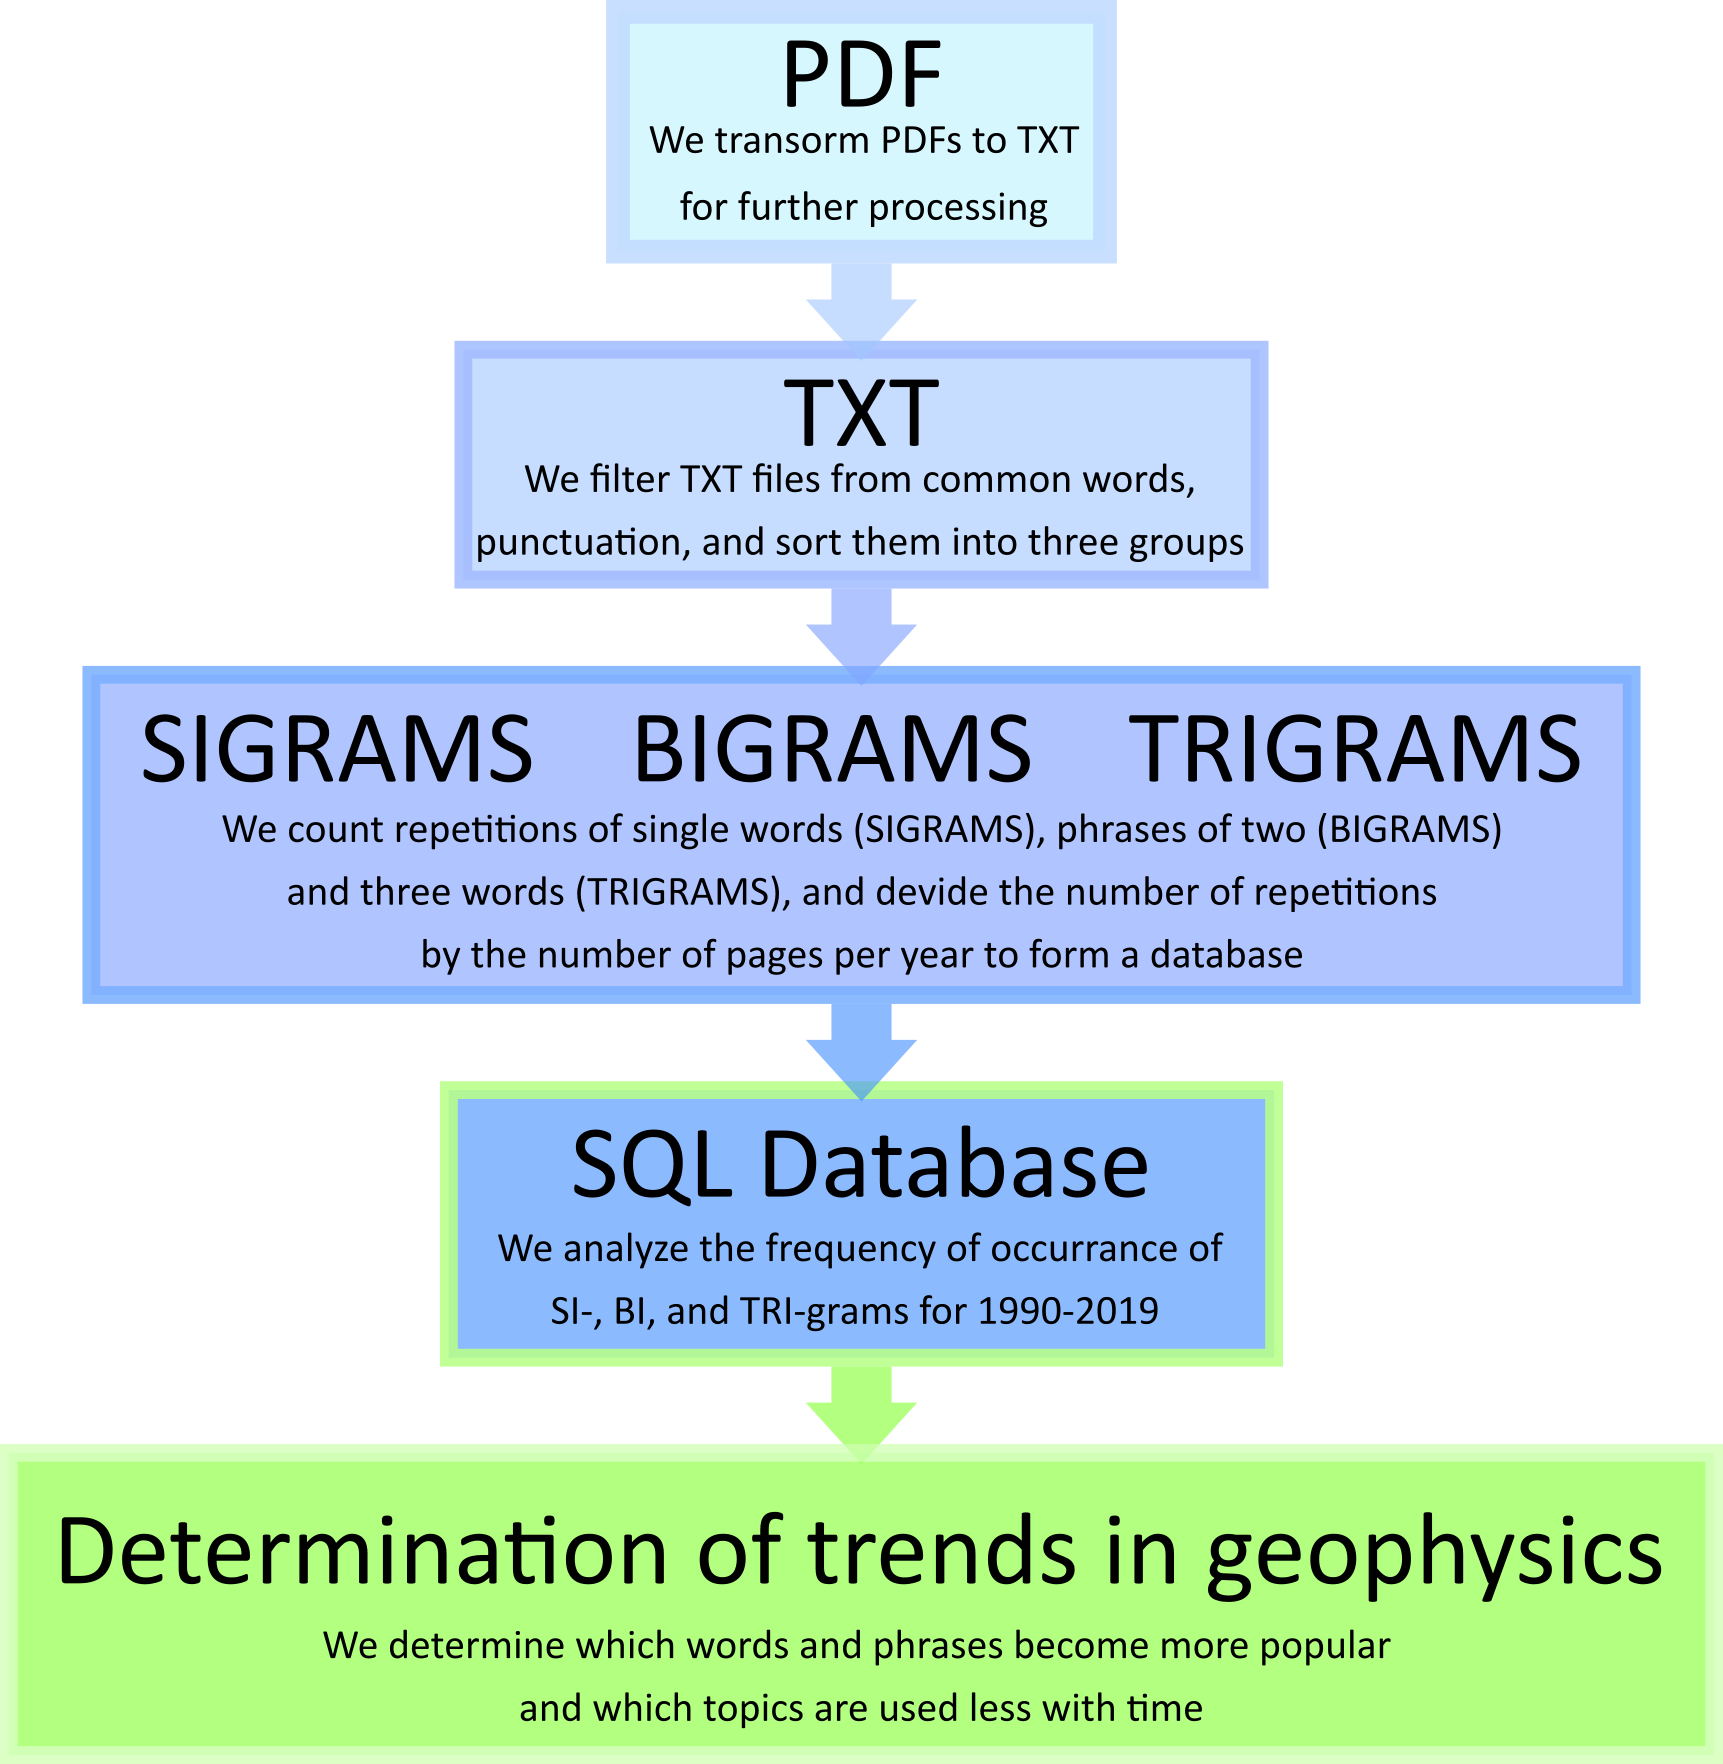
\includegraphics[scale=1]{scheme.png}
\caption{Data processing workflow.}
\label{scheme_workflow}
\end{figure}


In total, we analyzed 24,500 papers consisting of more than 57 million words or more than 383 million symbols.

 
%%%%%%%%%%%%%%%%%%%%%%%%%%%%%%%%%%%%%%%%%%
\section{Results}

We present our analysis of manuscript texts from the SEG Annual Conference. However, instead of focusing on average text length or sentence complexity, we look into the technical side. For example, we analyze and compare the frequency of occurrence of technical terms, such as ``data'' or ``velocity.'' Such an analysis sheds some light on technology development and trends in the field.

The usage of the most frequently used English words (``the,'' ``of,'' ``and,'' ``to,'' \textit{etc.}) per page remains unchanged over the last three decades. Therefore, we normalize the data to the number of pages of all articles each year. Often pages are not entirely filled with text; there are many graphs and formulas. Moreover, we know precisely the number of characters used, and we can estimate the number of pages.
We calculate the average number of pages, $Np$, for each year using the formula: $Np_i = \frac{Ns_i}{3000}$, where $i$ is the corresponding year, $Ns$ - number of symbols, 3000 is the number of characters for the common one spaced web page. The estimated number of analyzed pages is 127.9 thousand.
When analyzing the graphs in the present paper, one can state the number of times the phrase occurred per page each year.

\subsection{Most common words and phrases}

Fig. \ref{grams} shows the most commonly used words, two- and three-word phrases that appeared in conference materials from 1990 to 2019. The most frequent words are ``data,'' ``model,'' ``velocity,'' ``seismic.'' Throughout the whole period of the study, the word ``data'' was mentioned more than 377700 times, ``seismic'' 252400, ``model'' more than 251500 times, and ``velocity'' more than 223300 times in thirty-eight years. Comparatively, the word ``that'' was mentioned 324240 times Most of the three- and two-word phrases are devoted to seismic exploration and seismic data processing. 

The frequent use of these words tells us that most of the articles are about seismic exploration and seismic data processing. The terms ``wellbore'' and ``logging'' were more popular during the 1980s, and now their relative occurrence is declining. 

\begin{figure}[ht!]
\center{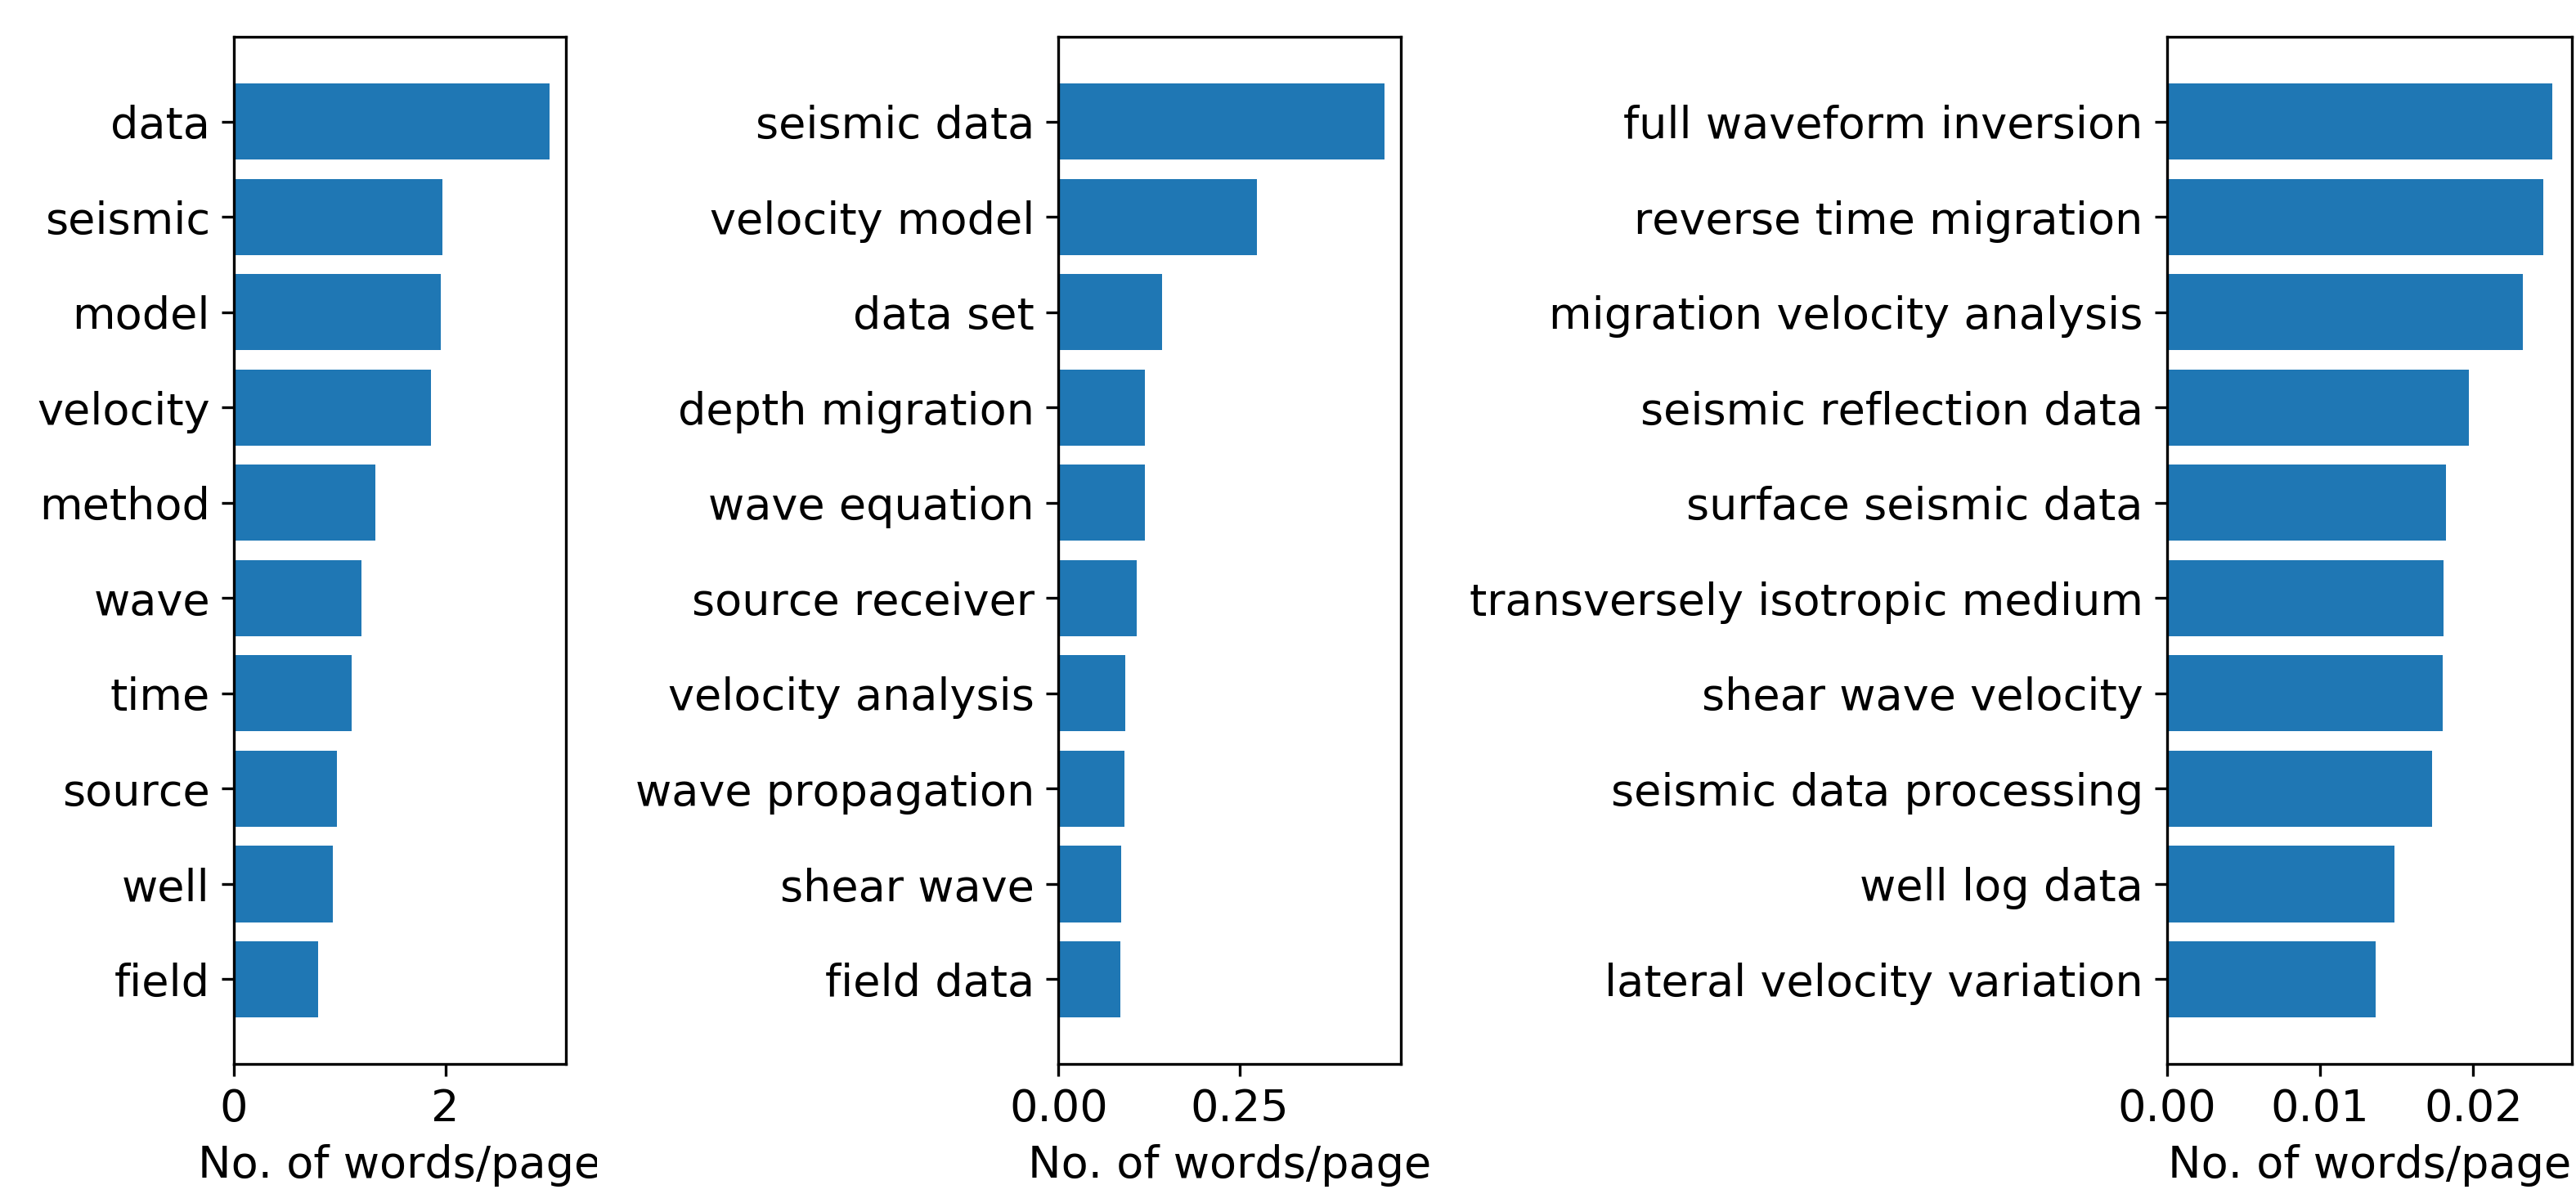
\includegraphics[width=\textwidth]{grams_hyst.png} }
\caption{The average frequency of single words (left), two-word phrases (middle), and three-word phrases (right) per page for the most frequently used terms (the 1990s-2019). The total number of pages is 127.9 thousand.}
\label{grams}
\end{figure}

While net average values provide information regarding the key concepts used over time, they are of less interest for absolutely the same reason. A more exciting approach is to monitor the evolution of other technical terms that constitute a subfield in geoscience or pertain to other disciplines. Such an analysis, however, is infinite. We limited the scope of this discussion to the objectives of the study, methods of data gathering and processing, shales, and neural networks. We also considered the fastest growing and declining trends in the publications.

\subsection{Objects of  Study}
Fig. \ref{rocks} breaks down the most used types of rocks. Each of the words on the left includes the most common names of rocks, e.g., sedimentary: shale, sandstone, conglomerate, carbonate, etc.; igneous: granite, diorite, basalt \textit{etc.}; metamorphic: gneiss, phyllite, slate, \textit{etc.} It shows the relative distribution of the objects of study: the majority of research deals with the sedimentary rocks. Terms that describe igneous rocks are used about ten times less than sedimentary, and the least used are metamorphic rocks related terms. The right part of Fig. \ref{rocks} shows the occurrence of rock types with time. The shale revolution starting in 2007 is clearly notable. The most occurring names of rocks are ``shale,'' ``sandstone'' and ``carbonate.'' We note how ``shale'' peaks around 2015 and starts declining afterwards. Besides, there is a steady increase in the appearance of ``carbonate'' (the 1990s - 2005), while ``sandstone'' is used evenly over the years. An attentive reader will notice that during the growth of the use of the word ``shale,'' the fluctuation in the use of the words ``sandstone'' and ``carbonate'' decreased.


We breakdown the sum of the names of geophysical methods used from 1990 to 2019, Fig. \ref{methods_objects}, left. They practically do not change over time, and we show the total in a pie chart. The whole pie chart is the sum of all the words we use in Fig. \ref{methods_objects}\footnote{Each of the words represents the sum of the related words: ``seismic,'' ``seismics''; ``magnetic,'' ``geomagnetic,'' ``aeromagnetic''; ``electromagnetic,'' ``em''; ``gravity,'' ``gravimetry,'' ``gravimetric''; ``electric,'' ``geoelectric''; ``logging,'' ``borehole geophysics.''}. We show the occurrence of the most common geophysical methods, and it gives us an estimate of SEG Annual Conferences content. Three-fourths of the material relates to the collection and processing of seismic data; the remaining quarter accounts for all other methods. We see that the primary method discussed at the SEG Annual conference is ``seismic,'' its usage is an order of magnitude higher than other methods and it is still growing in the frequency of occurrence. It is worth noting that the word ``seismic'' is mentioned about four times more often than the word ``geophysics.'' On the right part of Fig. \ref{methods_objects}, we breakdown the names of the main resources. We observe a slight increase in the frequency of the words ``gas'' and ``water'' from 1995 to 2015. Perhaps this is due to the increase in reservoir modeling related research. 
Figs. \ref{rocks} and \ref{methods_objects} show that for the last 30 years there are no significant changes in the use of geophysical methods and objects, with the exception of an increase in the frequency of occurrence of ``shale'' from 2010 to 2018 and a slight increase in the occurrence of ``water'' and ``gas'' from 1995 to present days.
Significant changes occur in the use of terms related to specific methods of geophysical survey and data processing. This will be discussed in subsequent sections of the paper.

\begin{figure}[ht!]
\centering
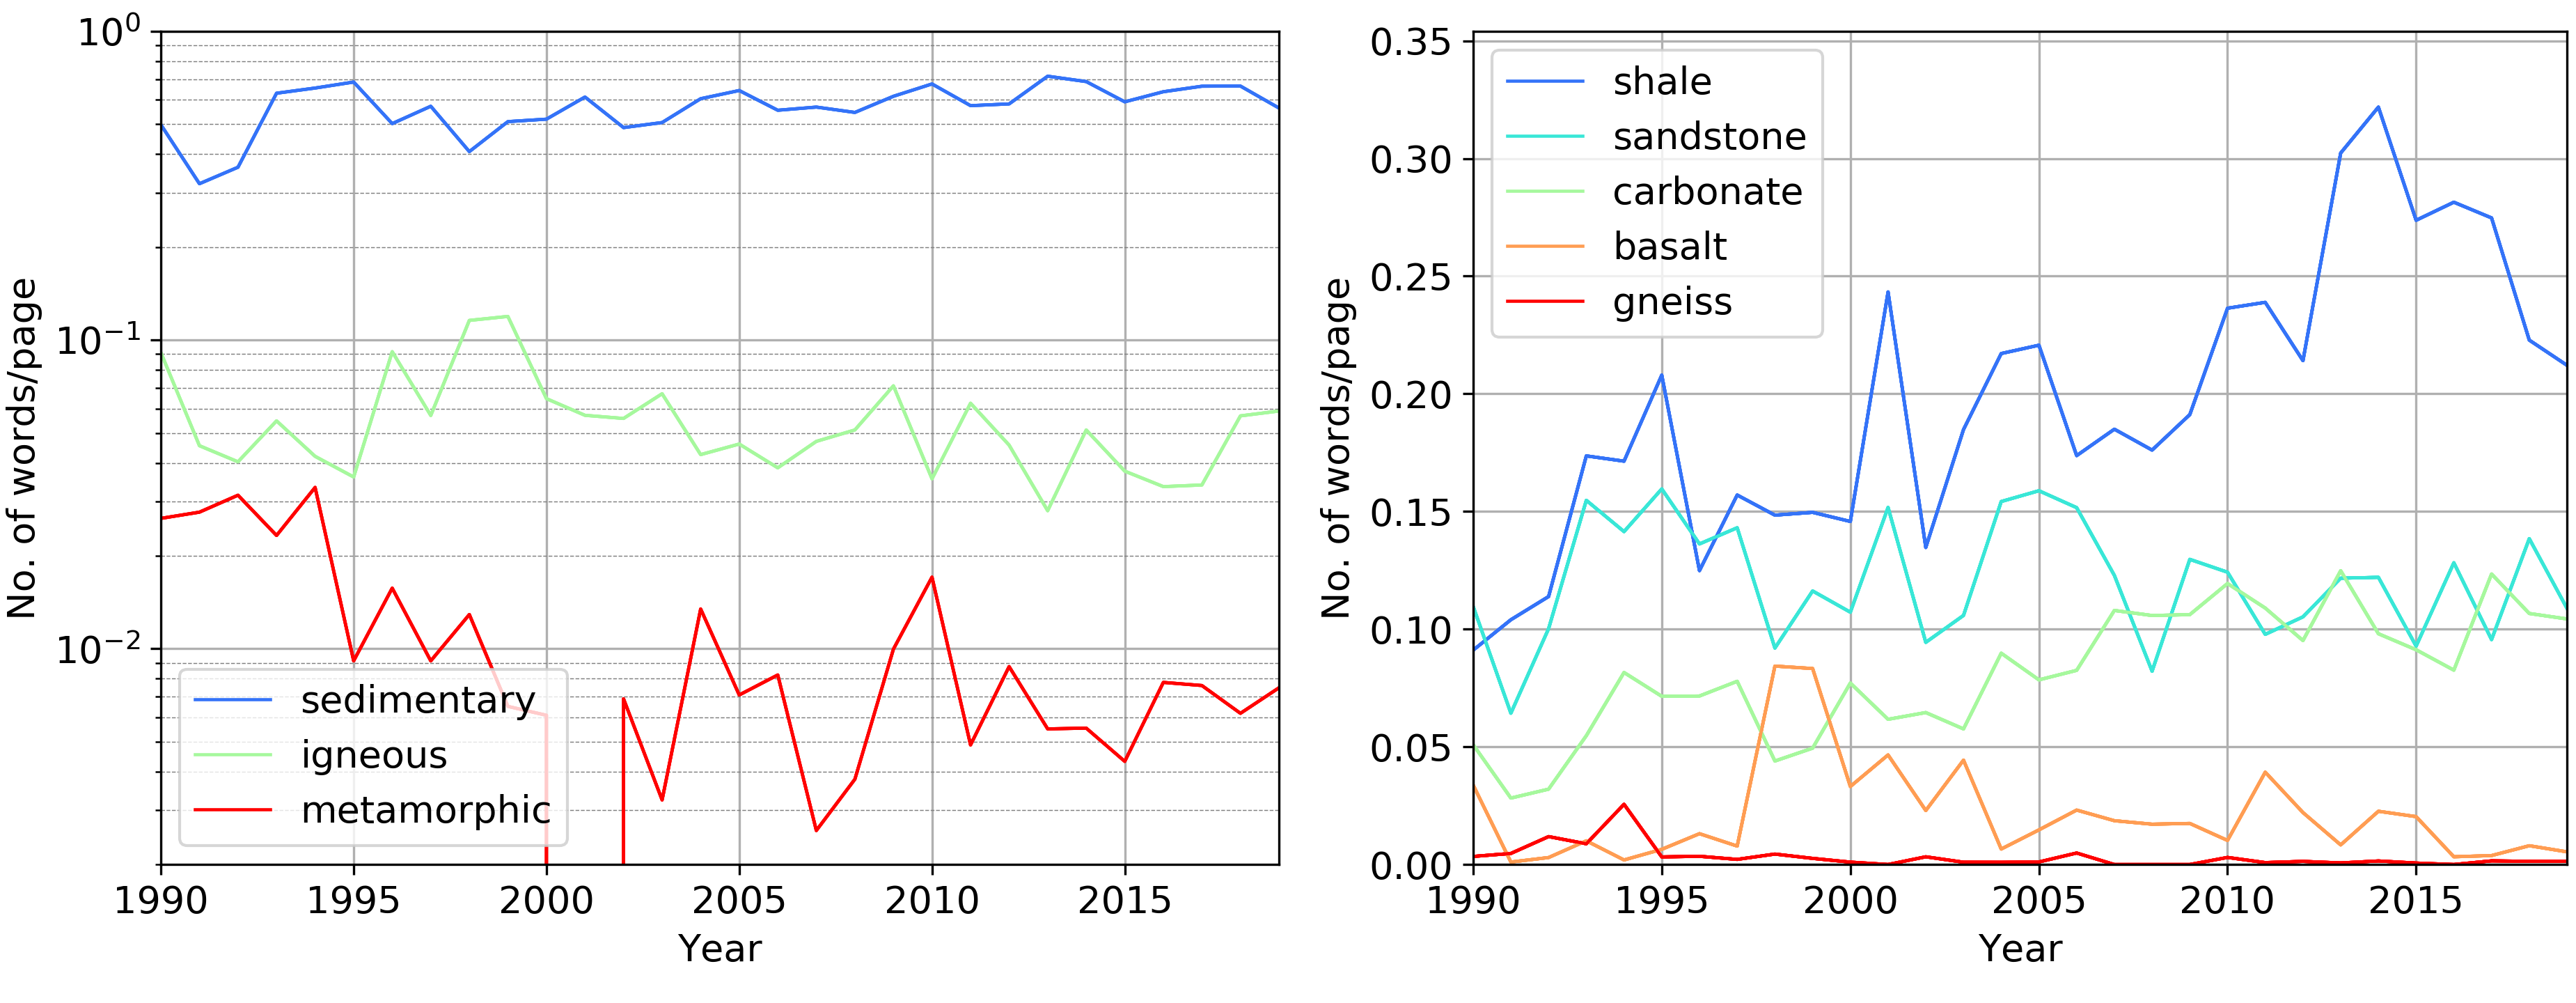
\includegraphics[width=\textwidth]{rocks.png}
\caption{Frequency of use of different rock type names (left) and most often used rock names (right). Rock types include most common rocks, e.g., sedimentary: shale, sandstone, carbonate; igneous: granite, diorite, basalt, \textit{etc.}; metamorphic: gneiss, phyllite, slate, \textit{etc.}}
\label{rocks}
\end{figure}


\begin{figure}[ht!]
\centering
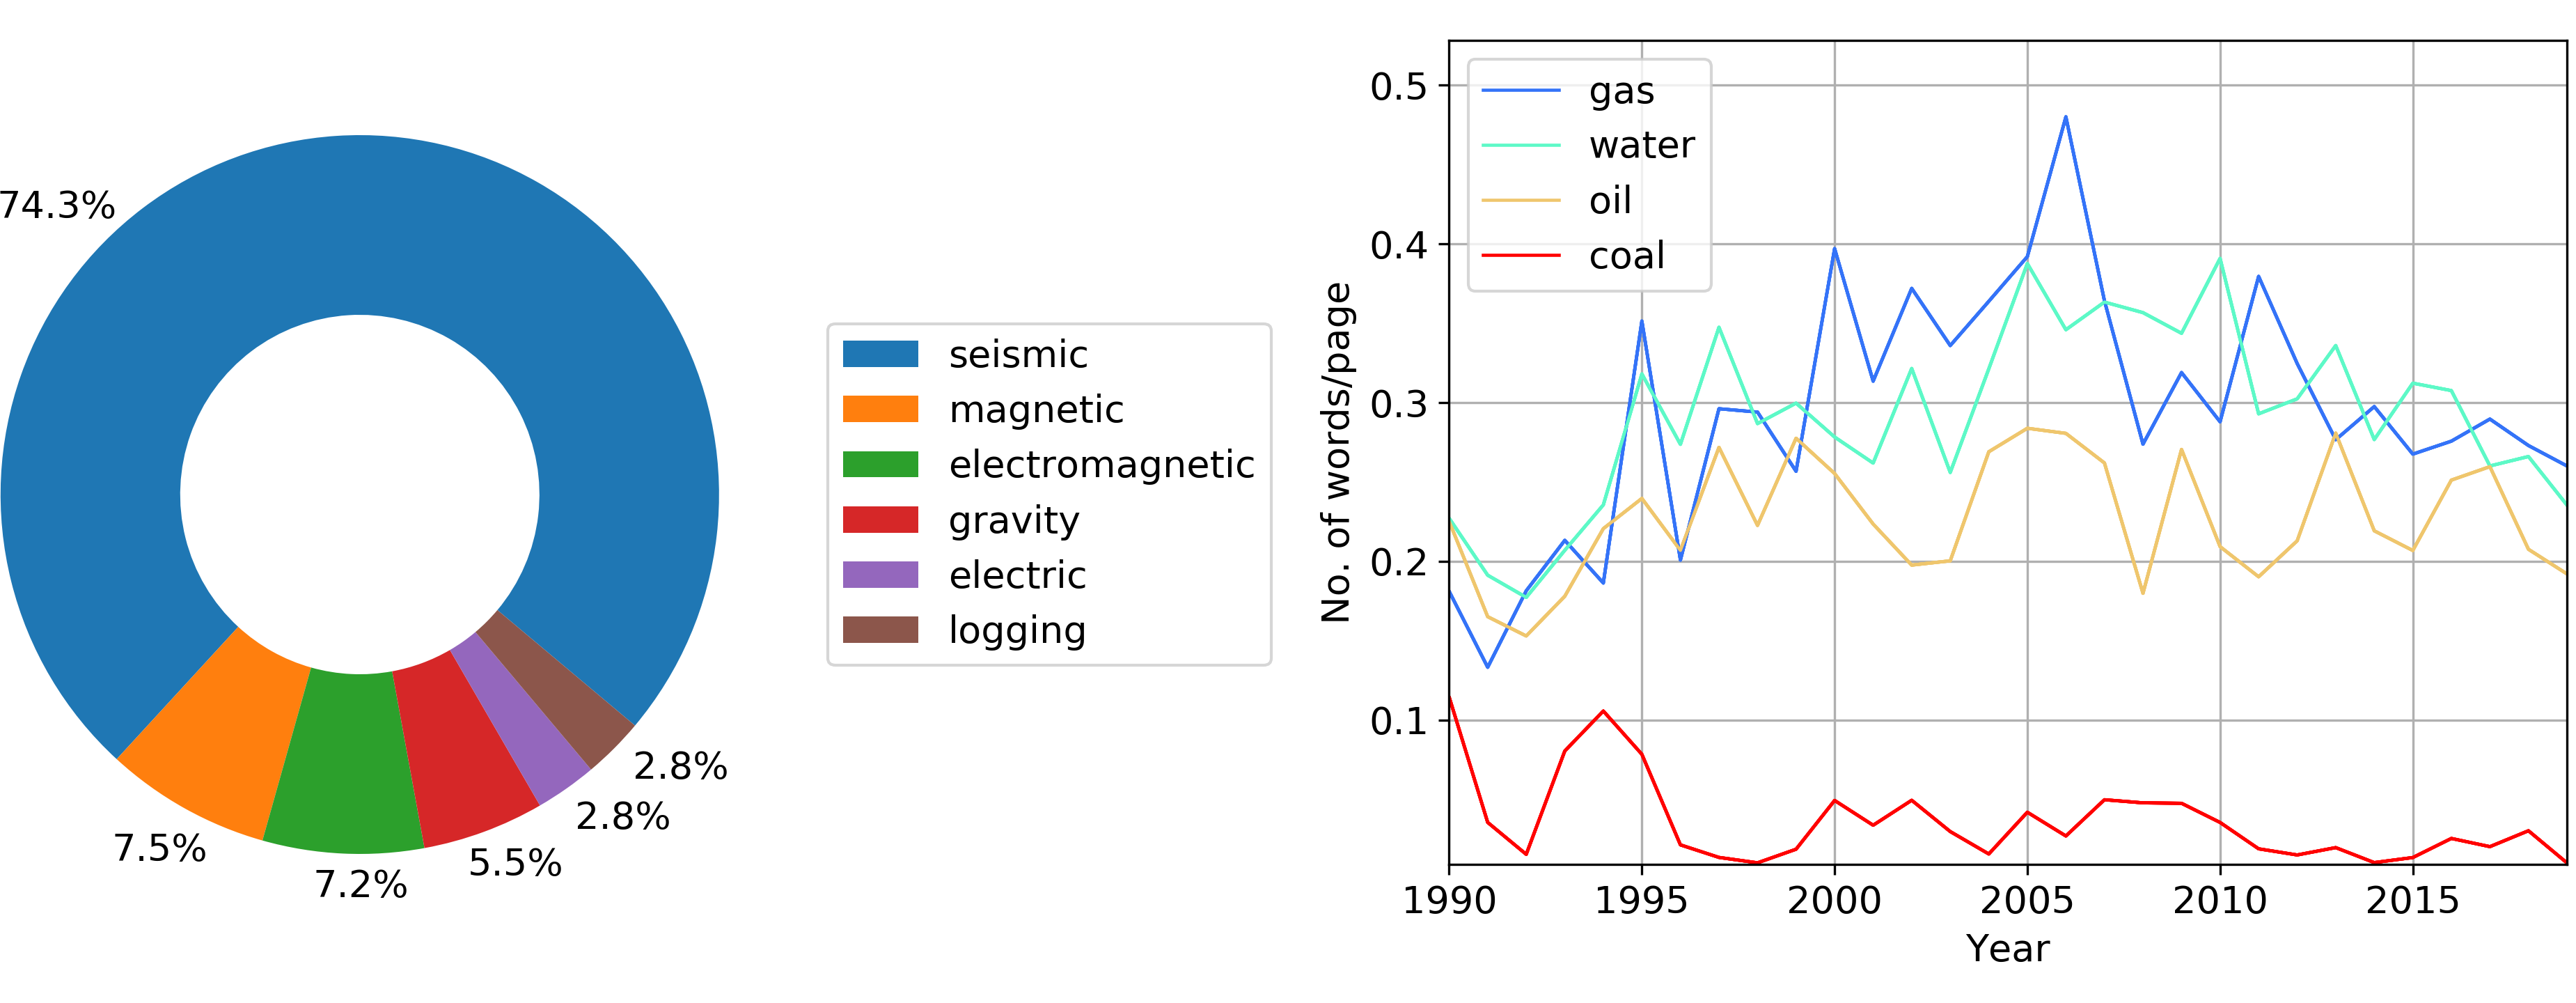
\includegraphics[width=\textwidth]{methods_pie_objects.png}
\caption{Geophysical methods of survey (left) and the most frequently used names of fossil fuels (right).}
\label{methods_objects}
\end{figure}

\subsection{Processing and data acquisition methods} 

Of all the three-word phrases, the most frequently used now is ``full waveform inversion'' (Fig. \ref{fwi_psdm}), and it is still growing together with the abbreviation ``FWI.'' The second one is ``reverse time migration,'' the 2019 top three closes with ``convolutional neural network.'' Fig. \ref{fwi_psdm} shows how the occurrence of ``prestack depth migration'' was surpassed by ``full waveform inversion'' and ``reverse time migration.'' The frequency of occurrence is higher if we consider abbreviations. It is interesting to note that the abbreviations ``FWI'' and ``RTM'' are used more often than ``PSDM'' even when it was much more accessible. Perhaps this suggests a tendency to reduce and simplify the terms. The growth of the use of some terms inevitably supplants other words, provided that the volume of published material is approximately the same. While reviewing conference proceedings for the 38 years, we found many terms that were popular before, but do not find application in the modern world. 
Fig. \ref{proc_meth}, left, breaks down other trends in seismic data processing algorithms. We see that ``machine learning'' appears in the SEG Annual Conference proceedings more often in the past few years. The occurrence of the word ``broadband'' started to increase in the early 2010s with a corresponding decline in 2016-2018; it began to grow again in 2019. Using a wider frequency range and inclusion of the low frequencies proved to contribute to better resolution, penetration, and inversion \citep{Kroode2013}. Besides, we see an emergence in the rate of occurrence of the ``Marchenko'' method. ``Marchenko'' is a set of data-driven methods that help us to project surface seismic data to points in the subsurface, it relates Green’s function from a virtual source inside a medium to the reflection response at the surface of that medium \citep{Lomas2019, Thorbecke2017}. ``Markov''-chain-based approach is able to account for the change in seismic response of damaged structures \citep{Iervolino2016}, and it correlates with the occurrence of the word ``seismicity.'' The term ``seismicity'' is used for induced seismicity risk estimation \citep{Weir2018}, mine development \citep{Barthwal2018}, and other applications. It is known that ``machine learning'' and ``neural networks'' have recently significantly developed towards image recognition. In seismic data processing is assumed to be really helpful with automatisation of the reflections tracking. We will devote a separate part of the paper to usage of ``neural networks.'' Fig. \ref{proc_meth}, right, shows classic methods of seismic data processing and related terms. We see the rise and decline in the appearance of these words in the last ten years, these methods were developed in the 1990s and now they have already been studied enough, and therefore their usage is declining. It should be noted that despite the decline in the number of occurrence of the words ``Kirchhoff'' (migration), ``CMP'' (Common Mid Point) gather, ``NMO'' (Normal Moveout), ``velocity analysis,'' and ``interferometry,'' all of them are used in industrial seismic. These words are still used quite often, but the time of research and development of methods associated with these words was the 1990s and early 2000s. The decrease in the frequency of occurrence suggests that research on this topic has decreased.


\begin{figure}[ht!]

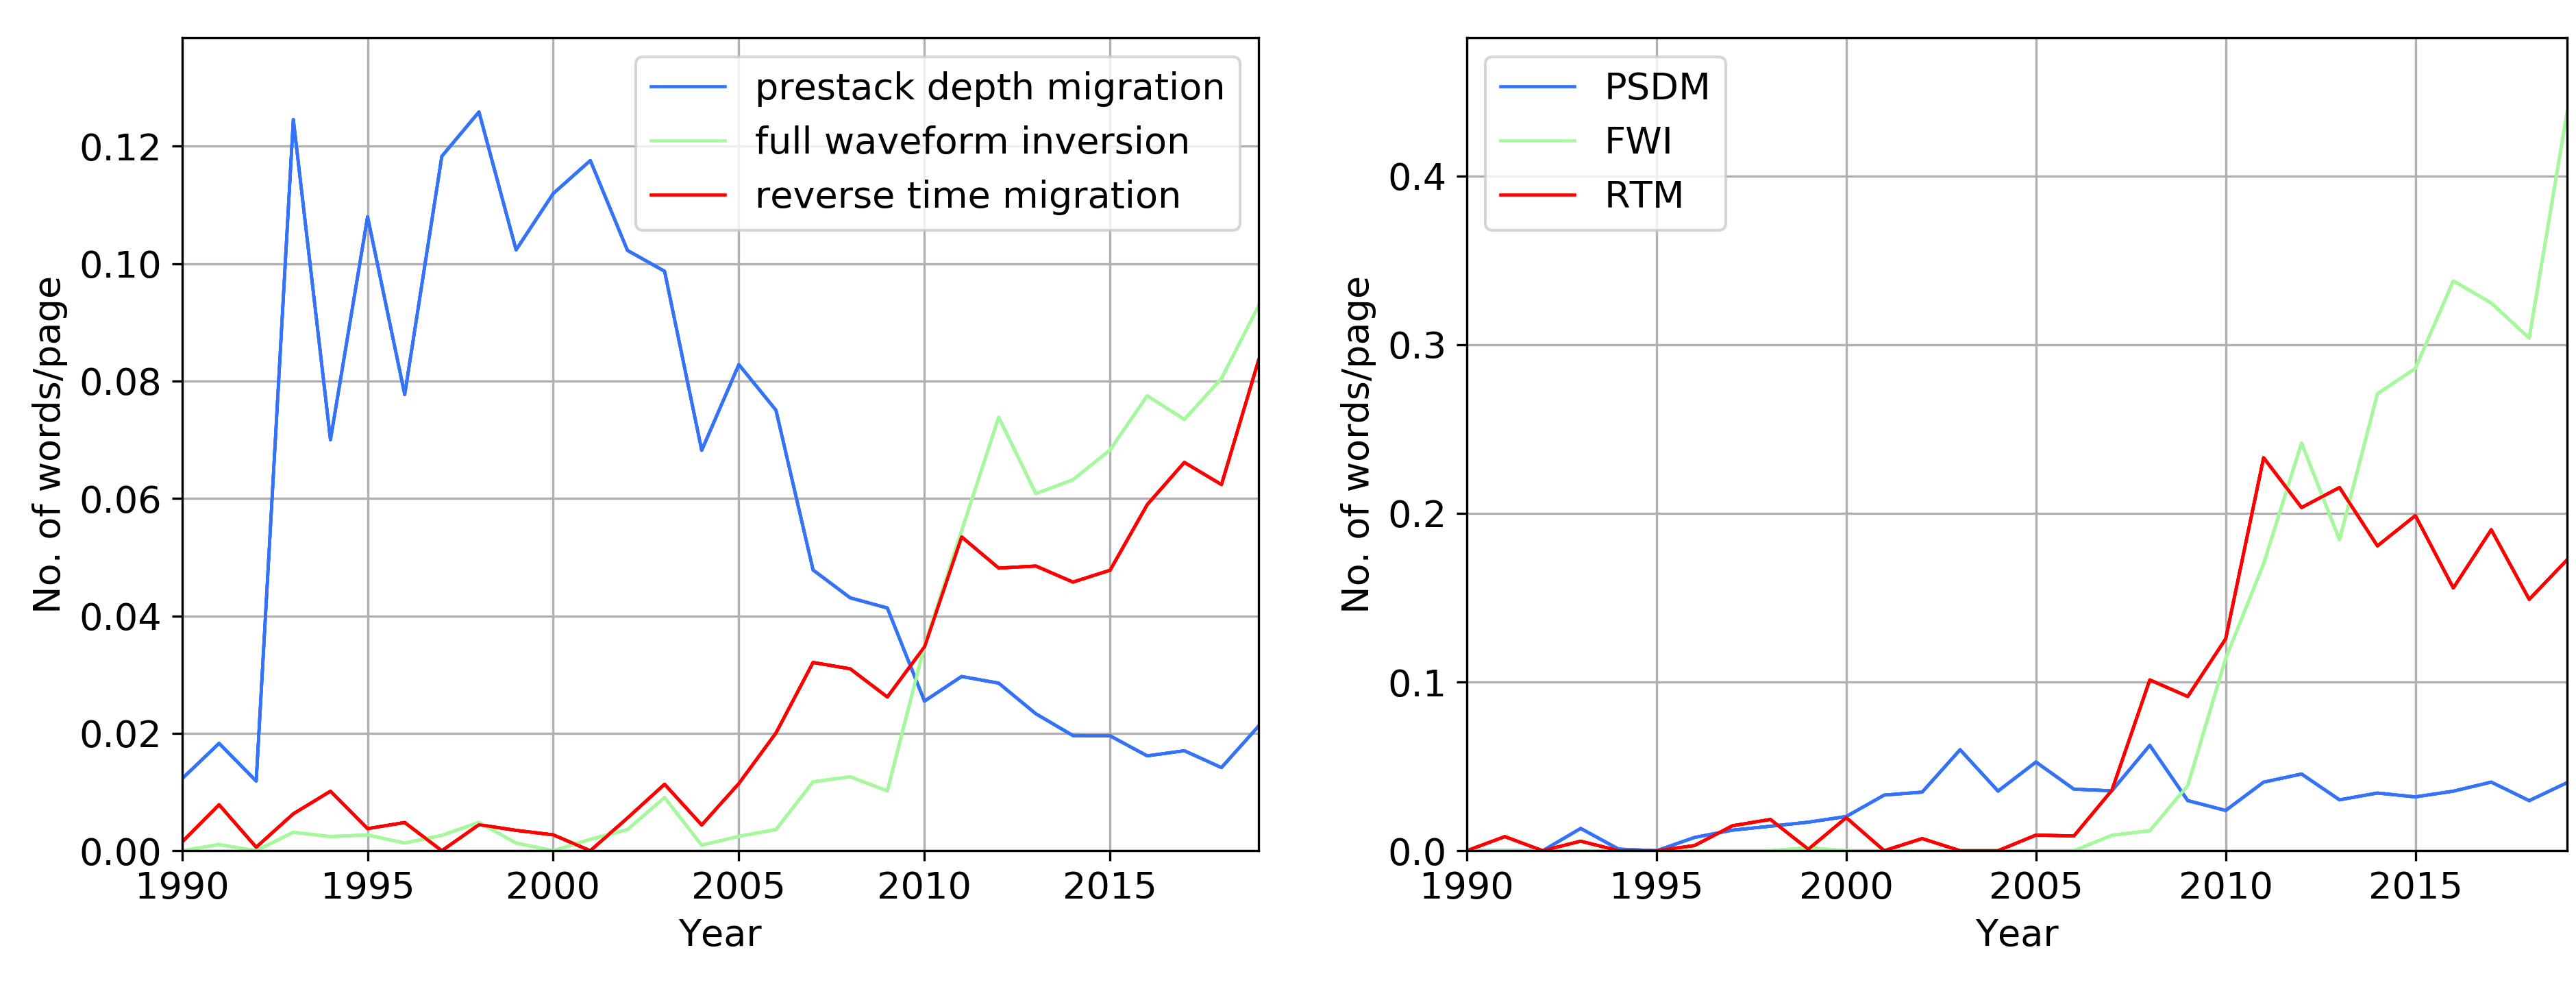
\includegraphics[width=\textwidth]{fwi_rtm_psdm_both.png} 
\caption{Change in the use of seismic data processing methods: full expression (left) and abbreviations (right).}
\label{fwi_psdm}
\end{figure}

\begin{figure}[ht!]

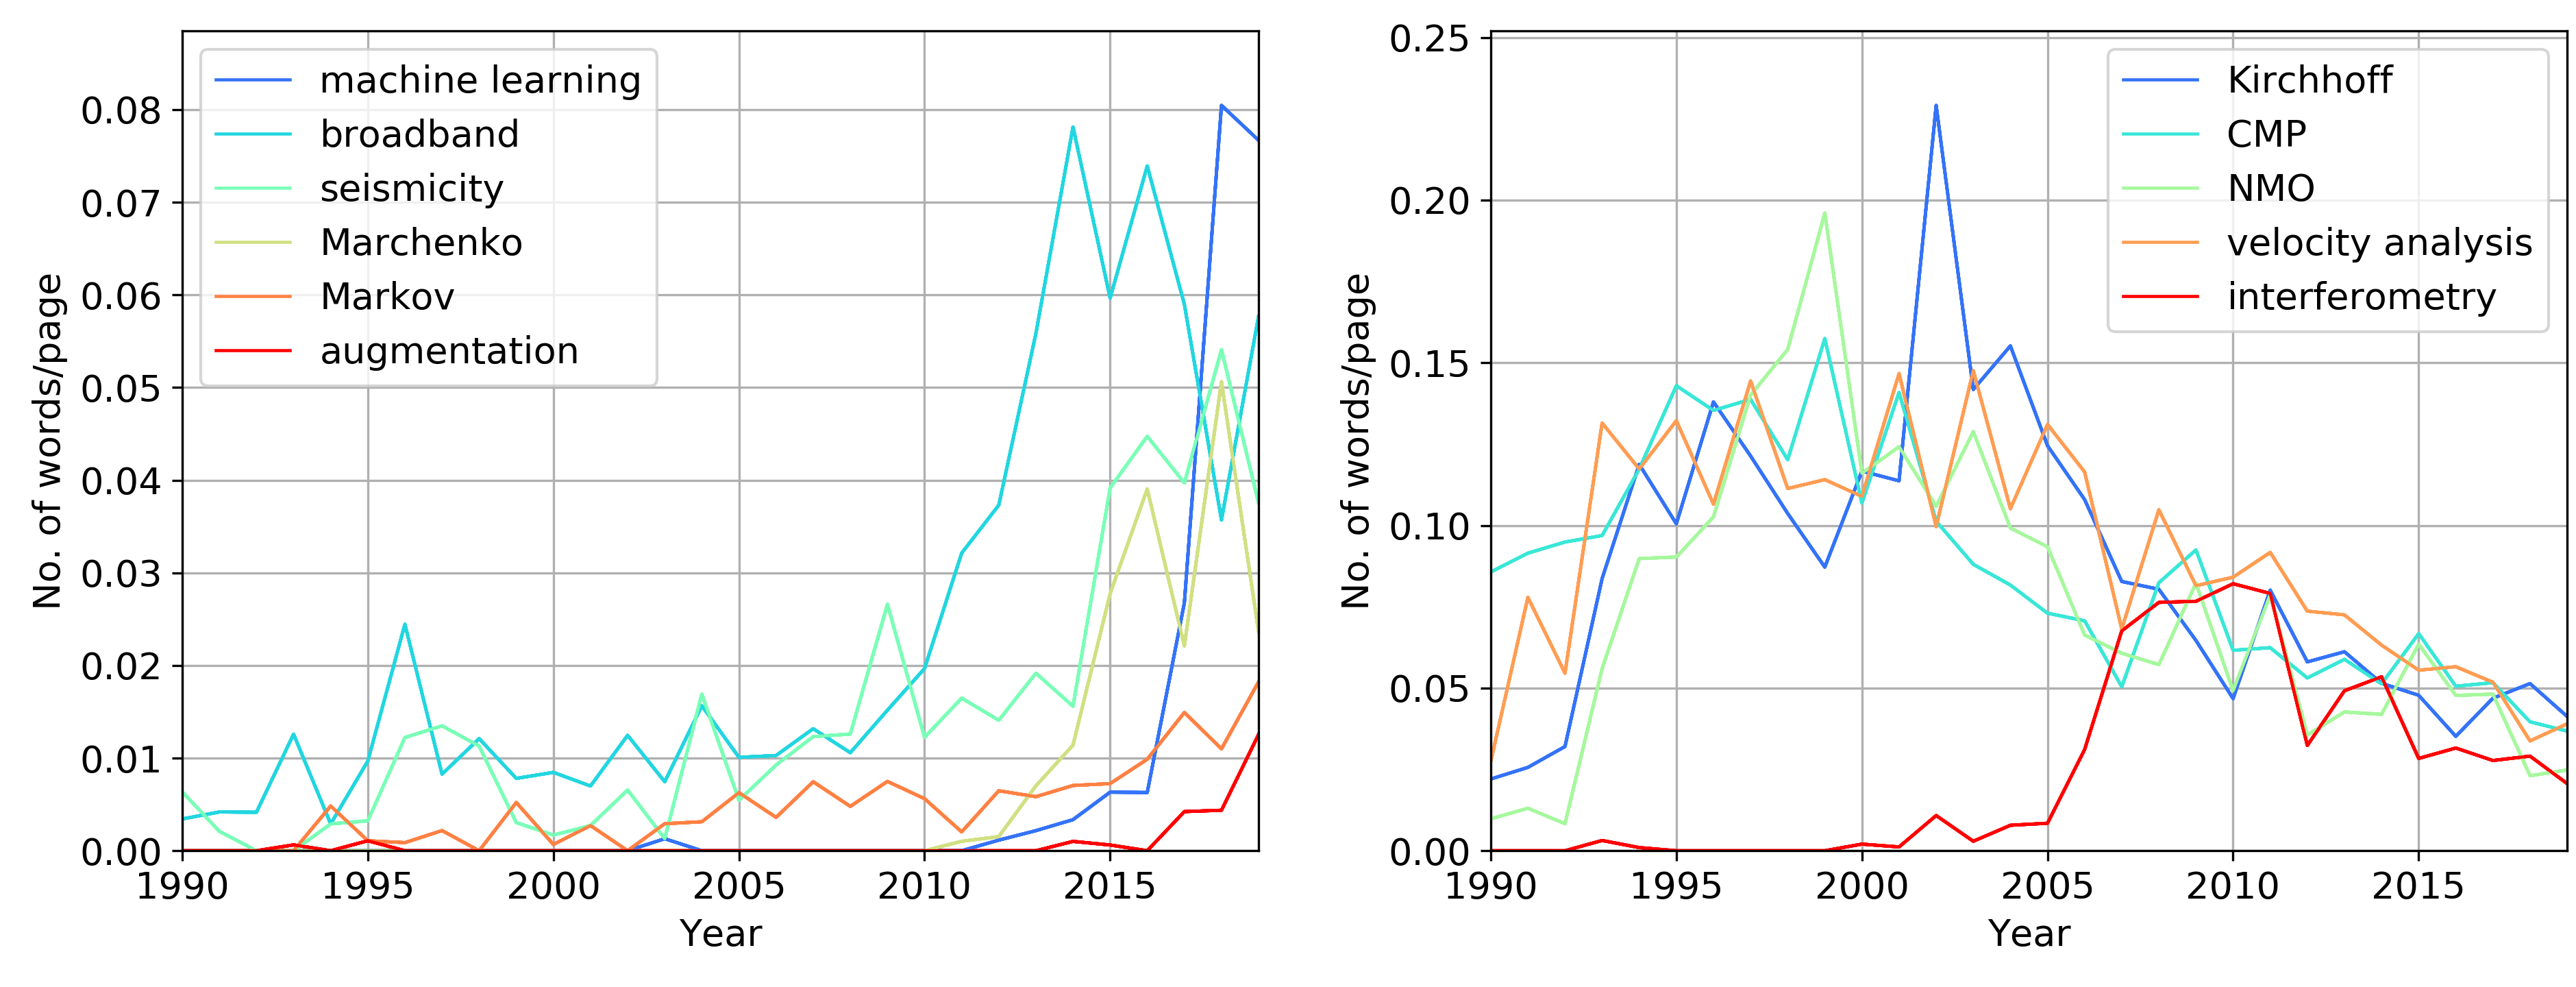
\includegraphics[width=\textwidth]{proc_meth.png} 
\caption{Trends in seismic data processing, terms, and algorithms that start to grow in usage (left) and decline in occurrence (right).}
\label{proc_meth}
\end{figure}




\subsection{Shale reserves} 
Fig. \ref{shales_frac} shows the most often used names of shale plays on the left, and ``fracking'' (includes ``hydraulic fracturing,'' ``frac,'' and ``fracking'') and ``shale gas'' + ``gas shale'' on the right. We observe peaking of shale-related terms from 2005 to 2015, which was followed by a decline in recent years. In the past 20 years, ``Barnett'' shale was mentioned more frequently than other shale deposits. In 2019 ``Marcellus,'' ``Eagle'' (Ford), and ``Barnett'' show the same occurrence, about one time per hundred pages. However, the term ``fracturing'' does not show such a fast decline. Despite the fact that the names of gas shale deposits reduced in use in the past three years, words that relate to the development and description of these deposits (``fracking,'' ``TOC'' - total organic carbon, ``unconventional'') do not show a decrease in use.


\begin{figure}[ht!]

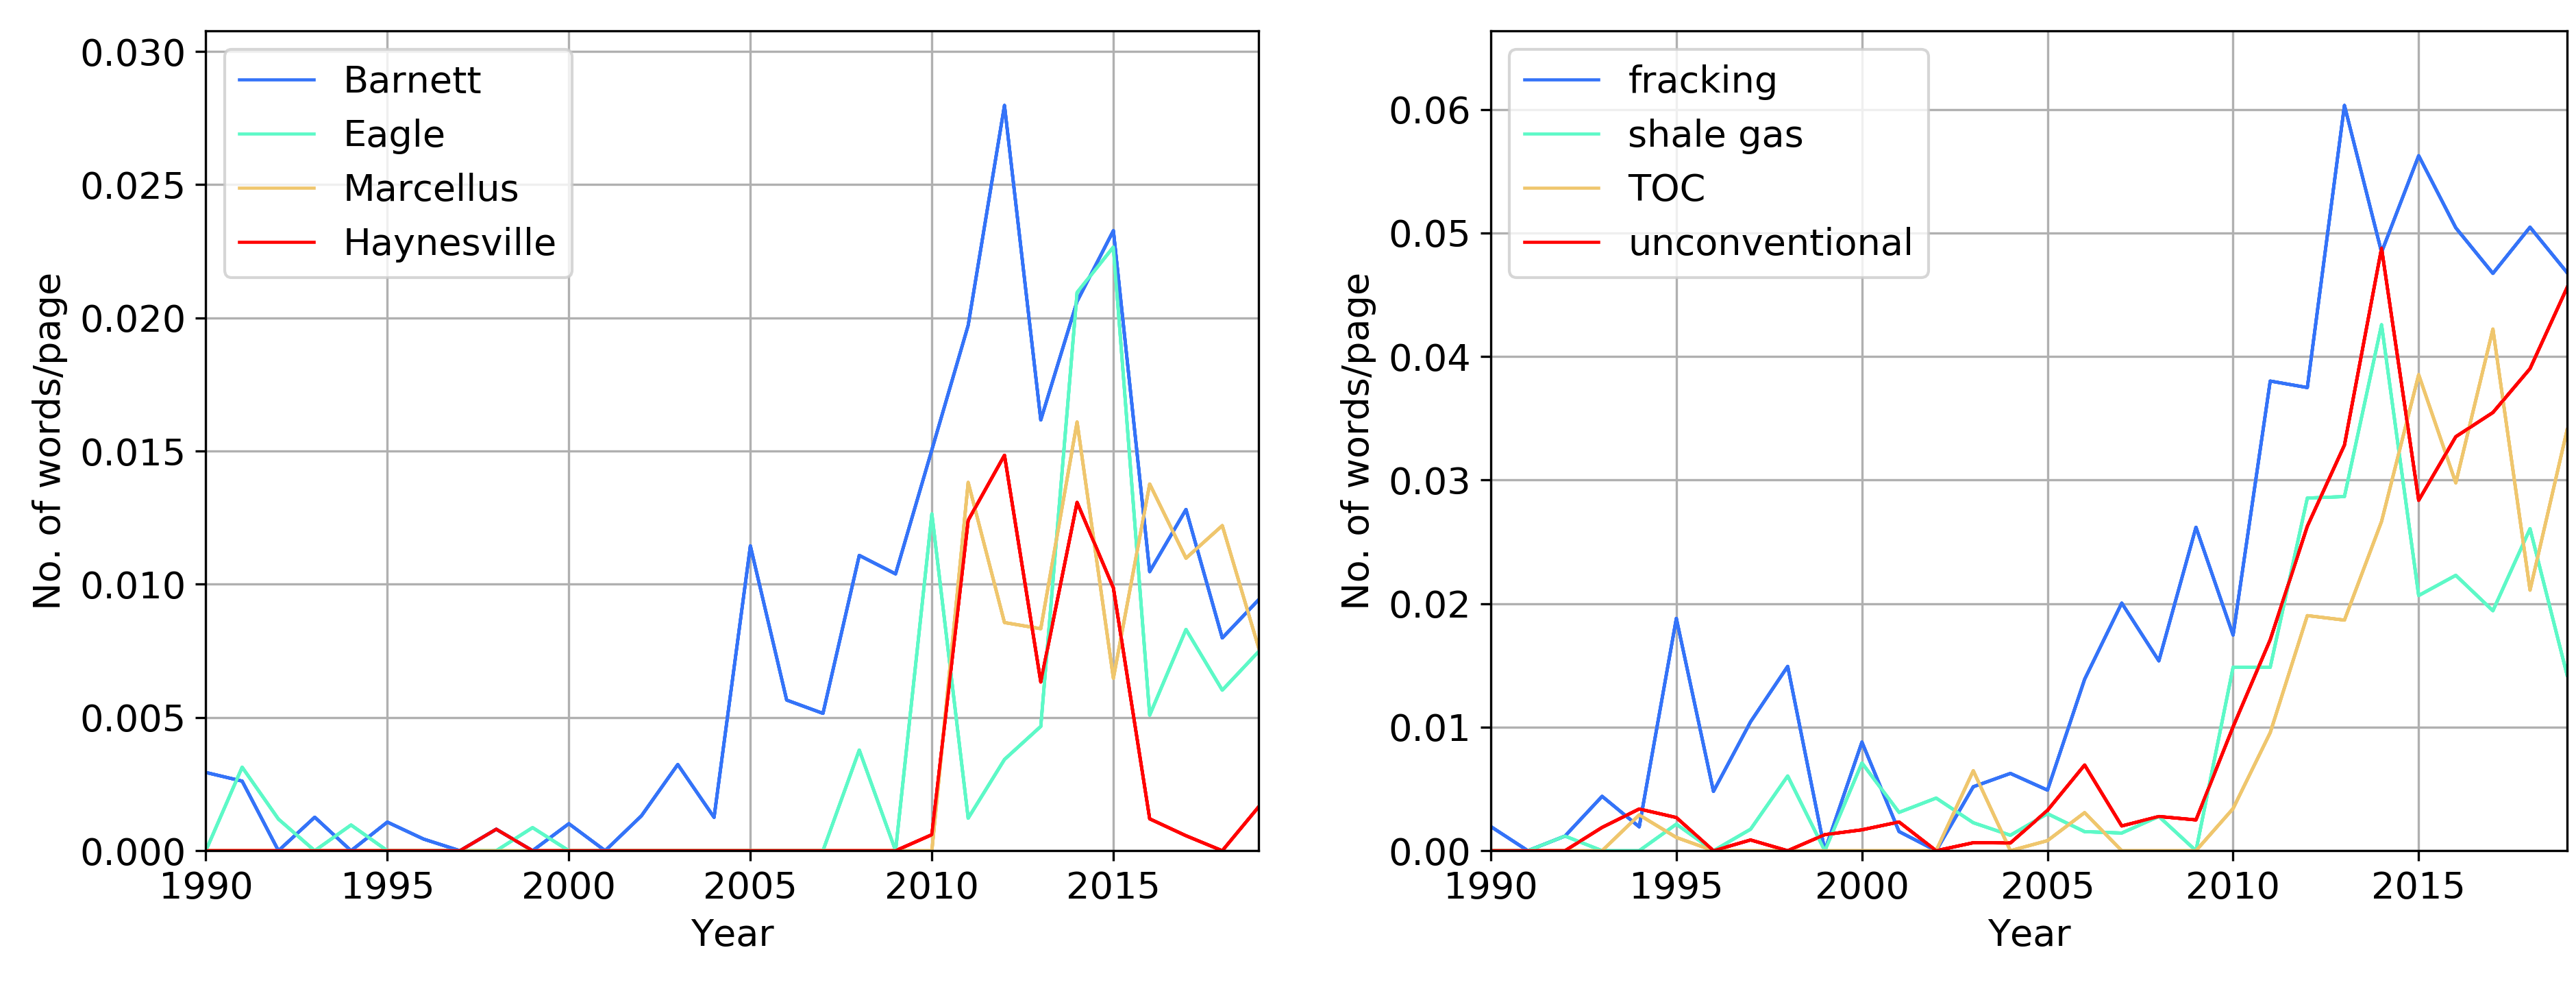
\includegraphics[width=\textwidth]{shale_frac.png}

\caption{Most frequently mentioned shale reserves; change in usage of hydraulic fracturing and shale gas.}
\label{shales_frac}
\end{figure}

\begin{figure}[ht!]
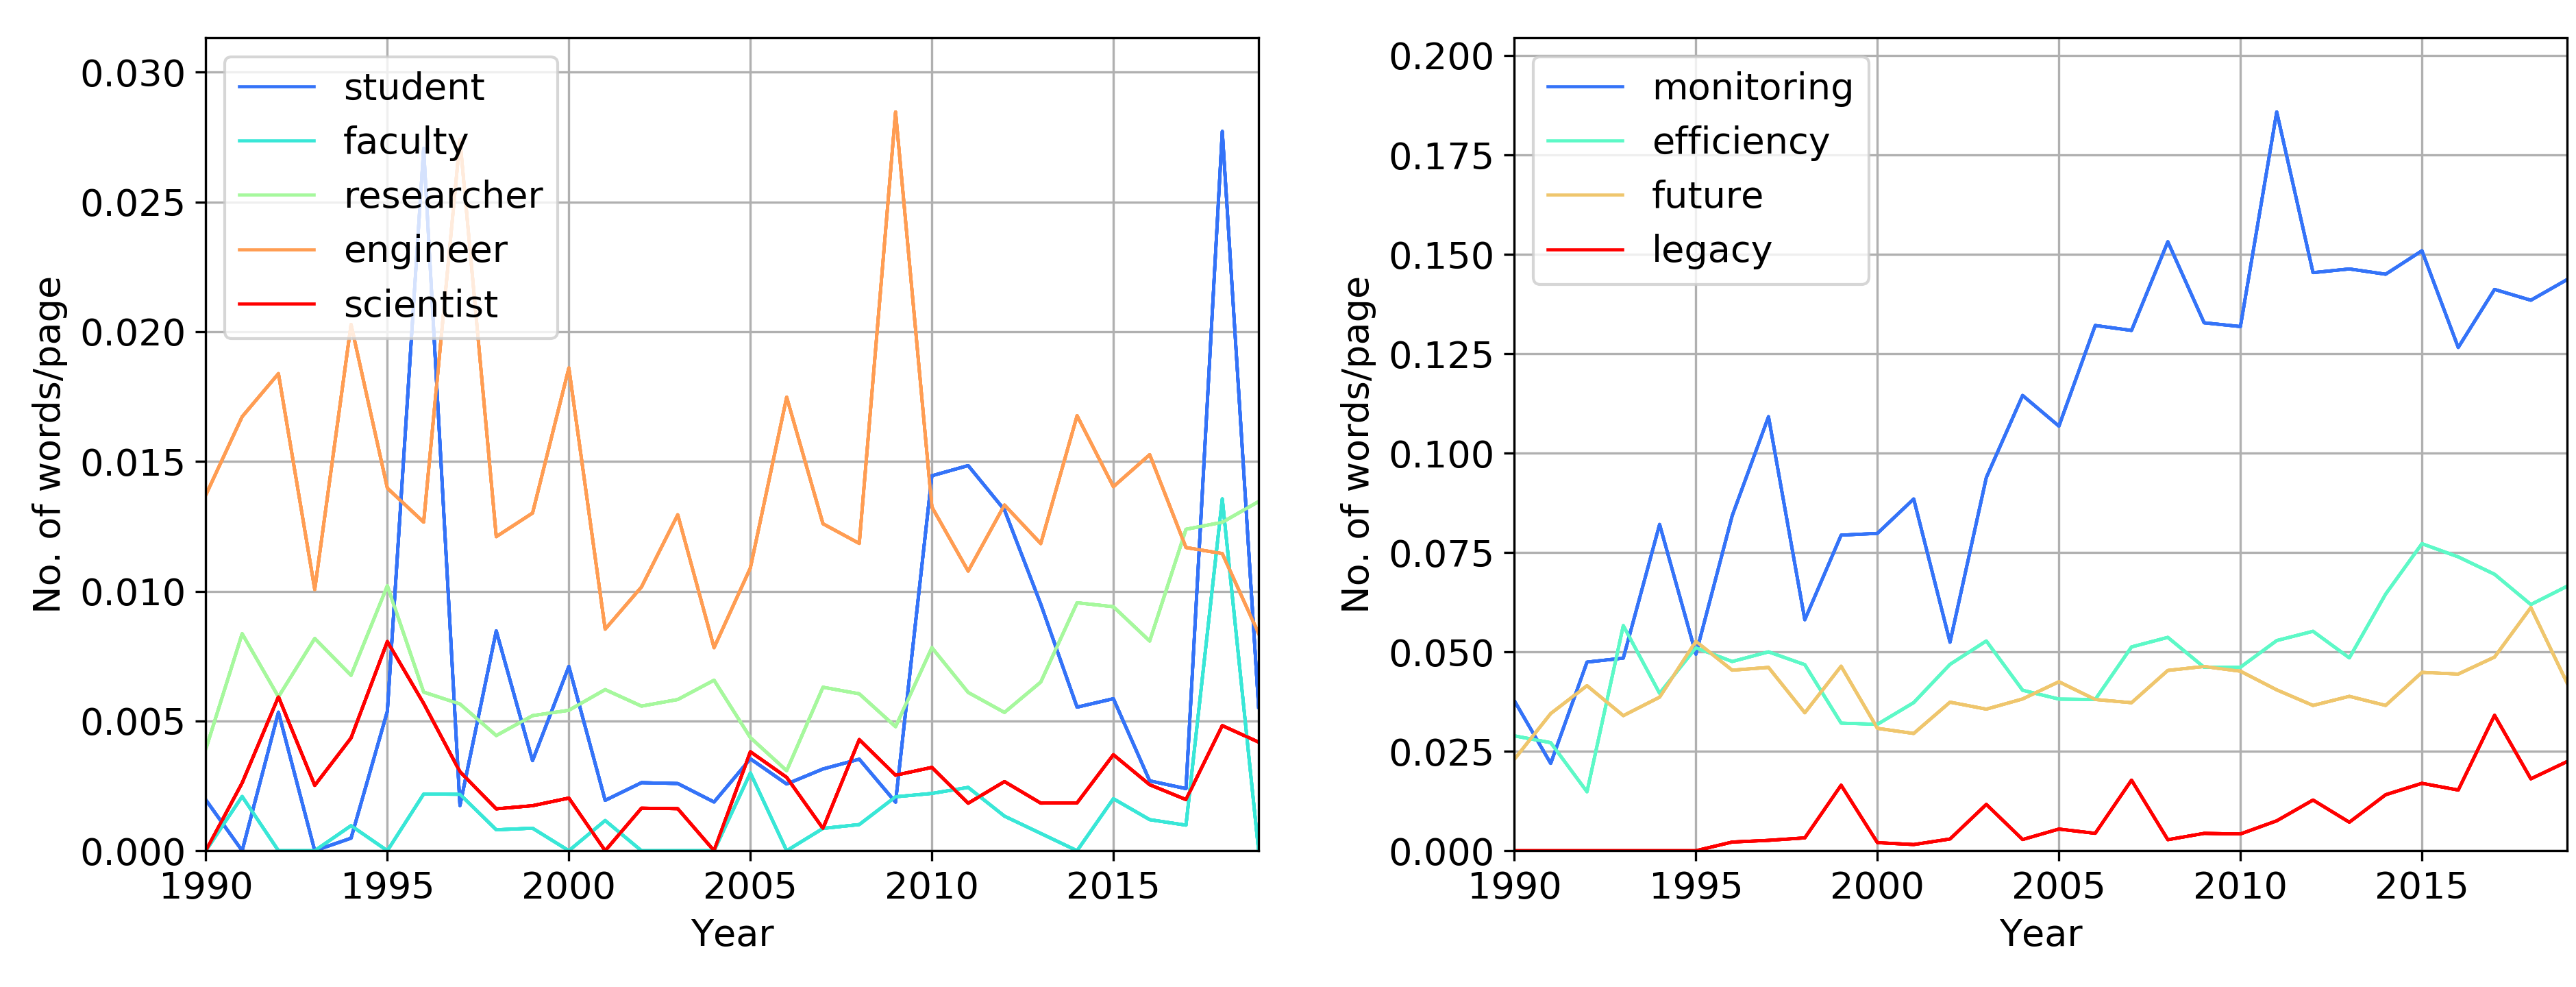
\includegraphics[width=\textwidth]{sigrams_int.png}
\caption{Change in word usage over time.}
\label{stu_faculty_mon}
\end{figure}


It is curious that in 2018, we observe an increase in the mention of the words ``student,'' ``faculty,'' and ``researcher," Fig. \ref{stu_faculty_mon}, left. Does this mean that the number of academic impacts has grown in the last year? You may notice the peaking of the word ``engineer'' after peaking of the word ``student.'' We observe the growth in frequency of the word ``researcher'' in the past ten years, and it appeared more often than ``engineer'' in 2019. During the 1990s, we see more of the word ``engineer'' in comparison to ``researcher'' and ``scientist,'' in the past decade, the situation has changed, bringing ``researcher'' to the first place. On the right side of Fig. \ref{stu_faculty_mon}, we observe an increase in the usage of the word ``monitoring.'' For example, this applies to microseismic monitoring and monitoring of the reservoir. The increased use of the term ``monitoring'' and ``efficiency'' indirectly indicates the concentration of researchers on the development of already explored deposits. The term ``legacy'' primarily refers to old data that is reprocessed using modern methods, including CNN. We used the word ``future'' regularly in the past 30 years, perhaps, we can agree, the past is over.


\subsection{Neural networks} 
We see that usually, the growth in the use of terms is saw-like; it is non-monotonic with individual peaks. Each peak represents the next phase of implementation, new research objects, and new teams that have mastered the method. ``Neural networks'' show a qualitatively different picture. From 1990 to the beginning of 2000, attempts were made to use neural networks in geophysics, but they were suspended until 2016, in which a rapid growth in the use of this and related terms began. On average, we find a ``neural network'' phrase on every fourth page of the conference materials. If we observe an increased interest in this topic, then the researchers sincerely believe that using the methods of machine learning can solve many problems of geophysics. Given this context, we pose the question: is the automation of geophysical data processing the main problem of modern geophysics? The authors believe that the main problem of geophysics is the lack of new research objects, such as hydrocarbon and other mineral deposits. Lack of survey objects is the reason for the increased interest in the development of methods for automatic processing of geophysical data. At the same time, the use of such words as ``monitoring'' and ``efficiency'' is growing, which indicates an understanding of the need for complete extraction of hydrocarbons and the monitoring of developed fields. Fig. \ref{neur_netw} shows the appearance of ``neural network,'' ``deep learning,'' ``artificial intelligence'' and ``field data,'' we use the last phrase for reference as it is always often used. In 2019, ``neural network,'' occurred more often than ``field data.'' It had already happened in 1993 and from 1999 to 2001, after that, it declined for a while, but now ``neural network,'' ``deep learning,'' and ``artificial intelligence'' have started to grow again ("artificial intelligence'' appeared during the 1980s). The question is: will the growth continue, or will it decline again as it did in 1993 -1995? The decline in interest in neural networks in early 2000 can be explained by an insufficient amount of computing power to realize the capabilities of the method. Now, technological progress allows us to use neural network methods successfully for face recognition. We also see attempts to introduce them to other areas of life. It is not necessary to be a rocket scientist to understand the reasons for the increasing interest in neural networks in geophysics. Experts want to automate geophysical data processing as much as possible. It remains only to be seen whether we need to automate seismic data processing deeply. With time, we will have fewer oilfields to be explored, providing space for monitoring and increasing production efficiency.

\begin{figure}[ht!]
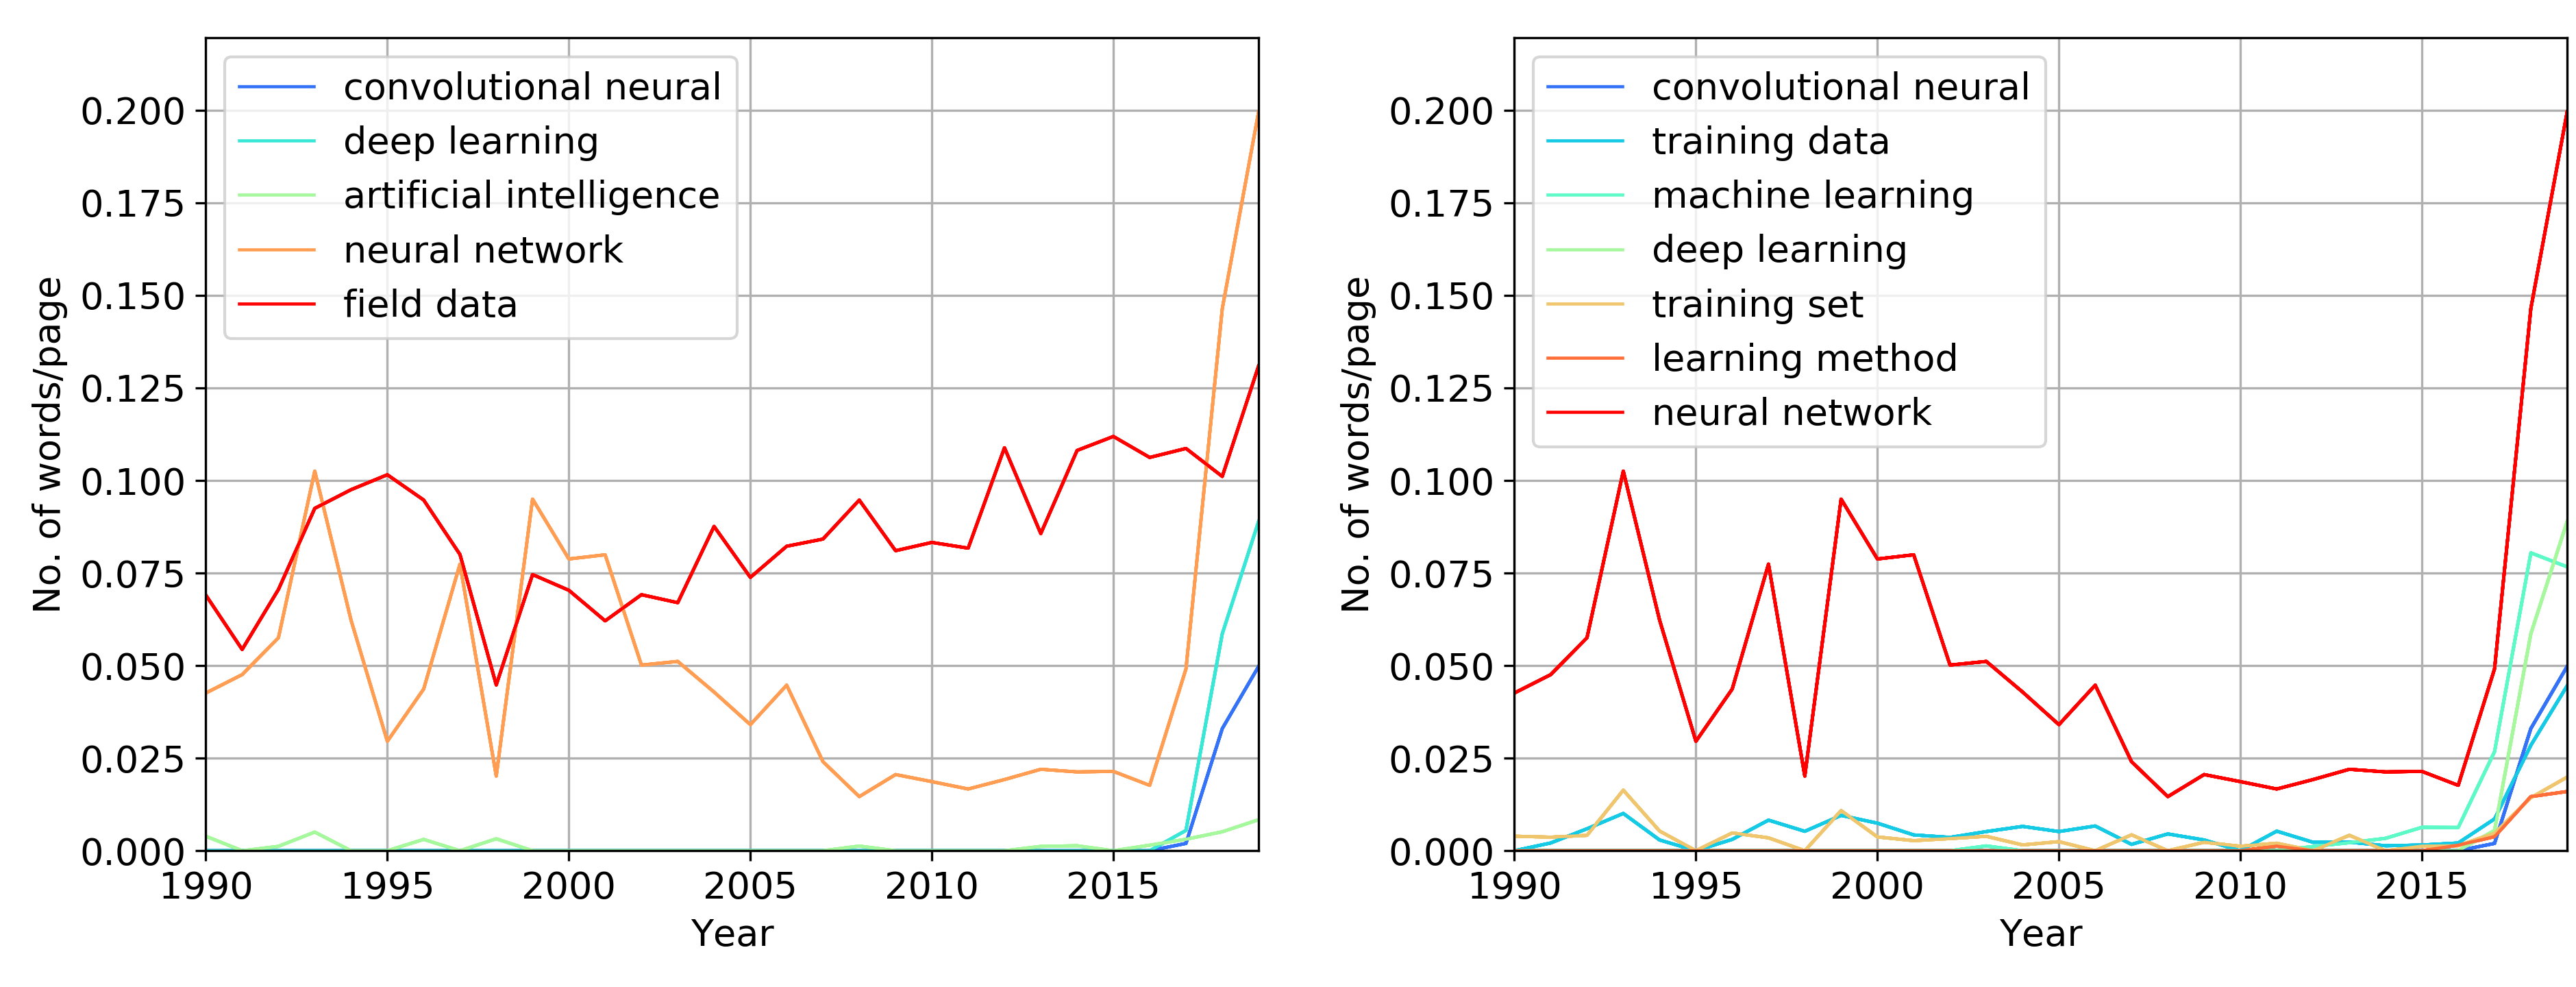
\includegraphics[width=\textwidth]{nn_related_all.png} 
\caption{``Neural network'' related two-word phrases. We display the phrase ``field data'' for the reference.}
\label{neur_netw}
\end{figure}


%%%%%%%%%%%%%%%%%%%%%%%%%%%%%%%%%%%%%%%%%%
\section{Discussion}

The emergence of new techniques in geophysics inevitably leads to an increase in the use of terms from this field. The frequency of the occurrence of words can be used to track trends in the equipment, processing methods, math algorithms, and types of resources, including oilfields and the kind of rocks under study. The amount of hidden information is astounding. Such a study is unique because we have at our disposal a history of the development of geophysics. Moreover, it allows us to track exactly how the professional language changes over time.


It is interesting to know the terms that are gaining popularity now and discover the current trends in geophysics. Fig. \ref{sigrams} shows words with the highest growth in occurrence on the left and highest rate of decline on the right. As one can observe, the majority of words that have grown in occurrence relate to the neural network method. Is it possible to assume that these words will continue to gain popularity in the years ahead and that the topic will remain relevant? For example, the phrases ``streamer em'' and ``receiver deghosting'' grew in occurrence at a very fast rate during 2011 – 2015, but since 2015, they have been declining as quickly as they were growing before. The word ``fiber'' and ``fibre''\footnote{``Chiefly British spelling of fiber'' \citep{MW2020}} is increasing in use almost as rapidly; this refers to fiber optics because seismic sensors based on fiber optics are now growing in use, because of their effectiveness in detecting faults filled with geothermal fluids \citep{Trainor-Guitton2018}, microseismic monitoring during hydraulic fracturing \citep{Binder2019} and other applications. The term “distributed acoustic sensing” (DAS) shows good correspondence with the word “fiber” as a DAS is based on fiber-optics, and these terms are closely associated. Here, the use of the word is directly related to the production of the corresponding equipment. For ``neural network,'' one can use the existing computing power. Per contra, the development of optical fiber requires production. However, in 2019, we observe a decline in the usage of the word ``fiber.'' ``Wasserstein'' (metrics) and (data) ``augmentation'' have also grown in occurrence in the past three years but as fast as ``Marchenko.'' In conclusion, that the lack of research objects forces professionals to develop processing methods and, for example, reprocess legacy data. The picture on the right-hand side in Fig. \ref{sigrams} shows terms that decreased in occurrence in the past four years.

Interestingly, there has been a reduction in the use of the abbreviation ``GPU'' by researchers as opposed to seven to eight years ago when the abbreviation was trending. ``Barnett'' shale is one of the most well studied shale deposit, and the authors believe that the fading of interest in it is a natural phenomenon. Curiously, there was increased interest in basalt at the turn of the century, and we observe increased interest in the early 2010s.


Besides ``neural network'' related terms (Fig. \ref{bigrams}) on the left side, we observe an increase in usage of ``tight sandstone'' and ``igneous rock.'' It is interesting to note that for 30 years, ``igneous rocks'' were rarely discussed, except in 2009. In 2018 and 2019, we observe several papers discussing igneous rocks found on Chinese and Brazilian oil fields. Their acoustic and elastic properties must be considered in reservoir characterization \citep{Penna2019}. On the right of Fig. \ref{bigrams} one can see two-word phrases that show a decrease in the frequency of occurrence in the past four years. When new research topics appear, new ones will partially or entirely replace old ones since the number of articles is limited each year. 

Hill first described Gaussian beam migration in 1990 \citep{Hill1990}. It is the seismic method that can image steeply dipping reflectors (more than 90 degrees) and will not produce unwanted reflections from the structure in the velocity model. In 1993 at the SEG Annual Conference, we observe several papers reporting usage of beam migration in seismic data processing. In 2001 we notice an increase in the number of occurrence of ``beam migration,'' with the increase in computing capabilities, it became possible to use this method for 3D AVO analysis (Amplitude variation with offset) of small and medium-size 3D seismic surveys \citep{Huang2001}. Interest in this method rises two more times, in 2008 and 2015. Frequency peaks appear with enviable regularity every seven or eight years. Moreover, each subsequent peak is higher than the previous one. In 1990, a new method appeared; in 1993, we observe testing on synthetic data; in 2001, professionals report the results of processing small and medium volumes of data, in 2007 and 2008, the results of use on large objects in the Gulf of Mexico \citep{Ting2008}, CGGVeritas. For 25 years, we have seen the emergence of new technology, testing, and application in field exploration. However, since 2015, we see a decrease in the rate of use of the phrase ``beam migration.'' The right part of the Fig. \ref{bigrams} shows a reduction in the use of other seismic terms and ``Barnett shale.''


\begin{figure}[ht!]

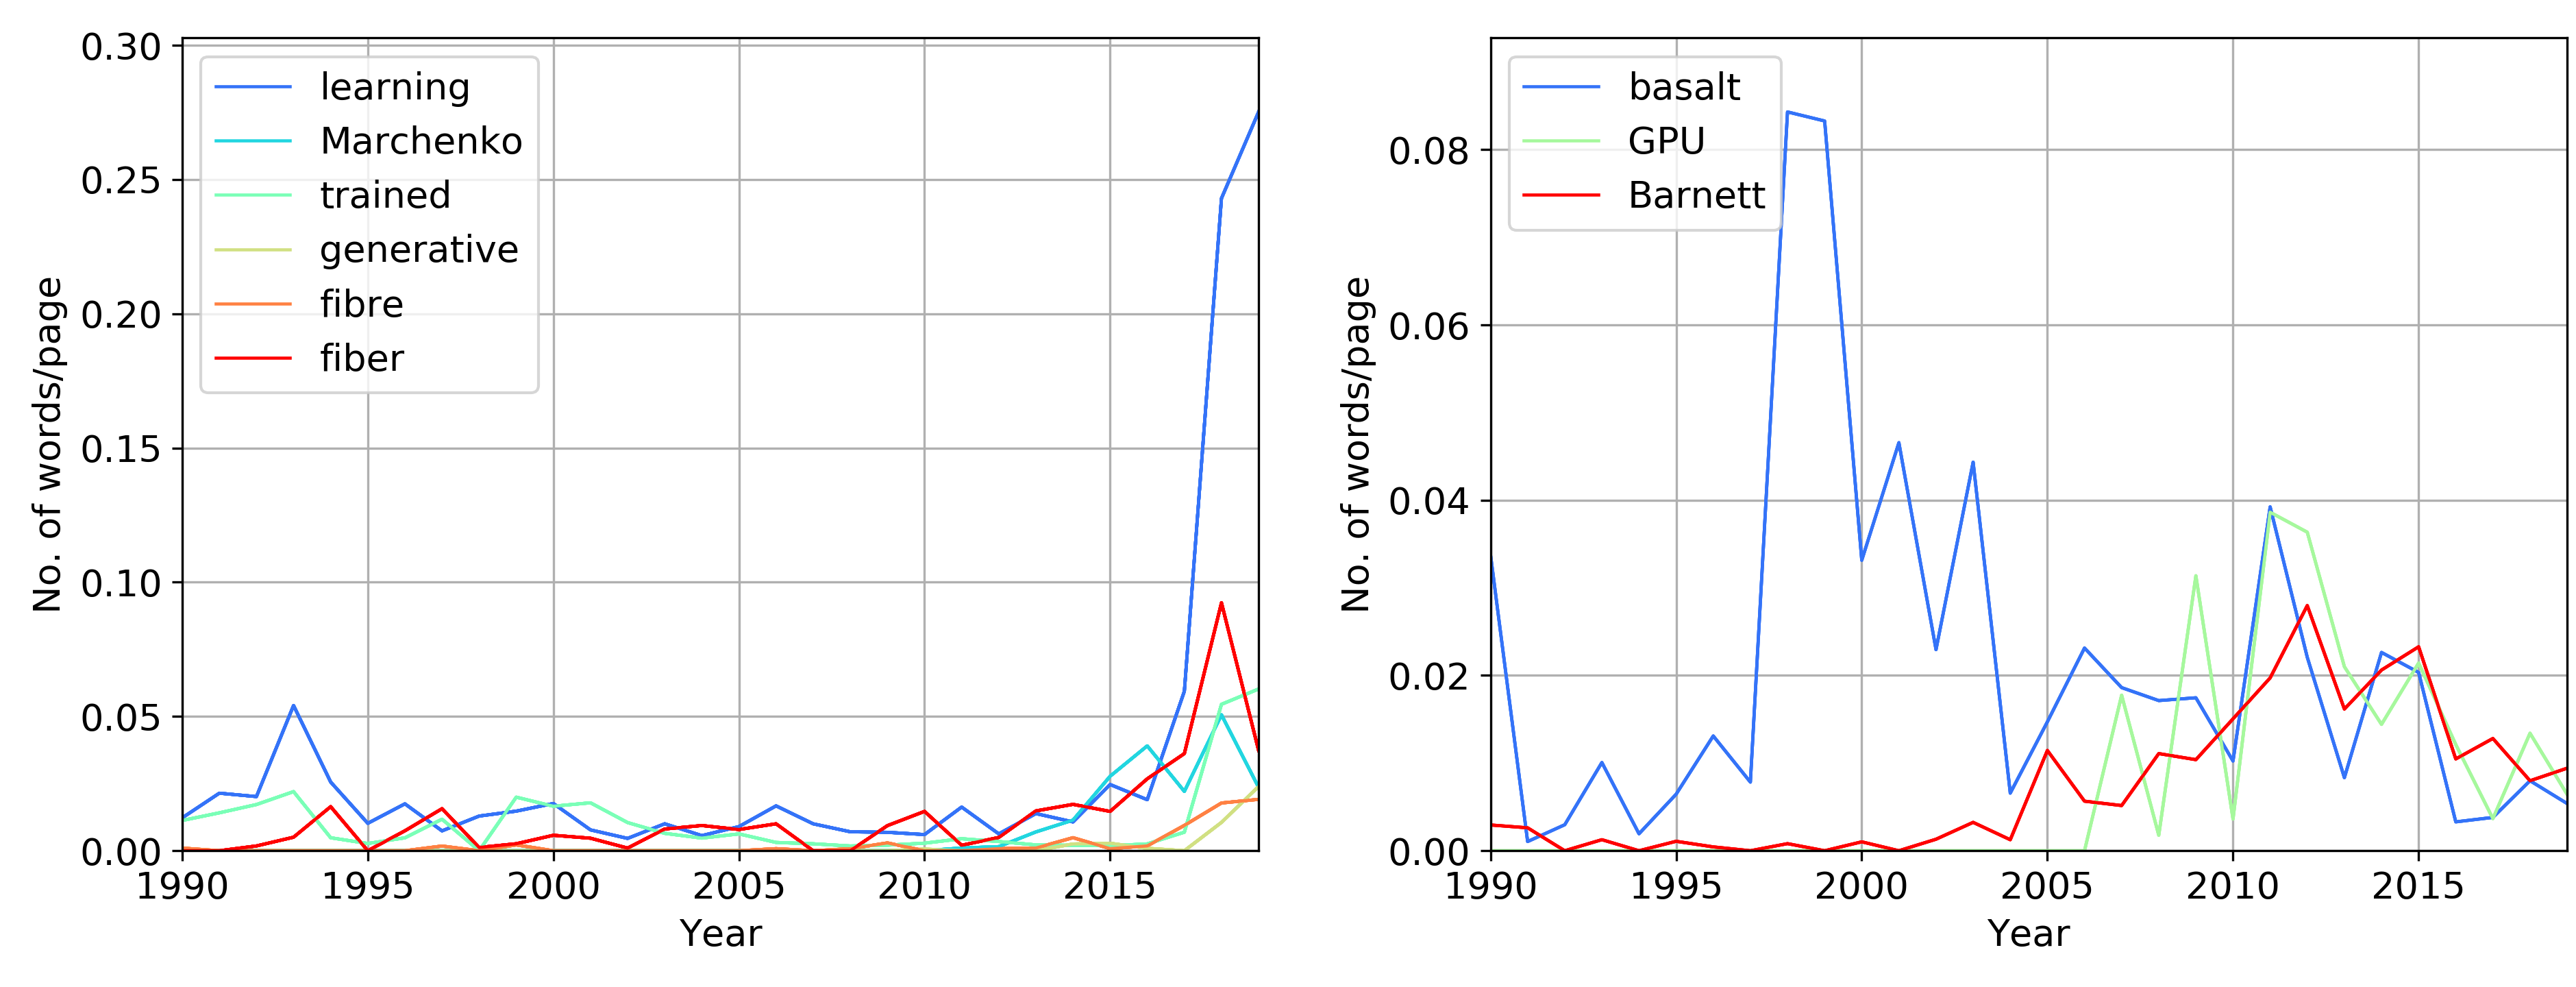
\includegraphics[width=\textwidth]{si_grow_decl.png}
\caption{Words that show the highest rate of growth in occurrence (left) and decline (right) in the past four years.}
\label{sigrams}
\end{figure}

\begin{figure}[ht!]
\center{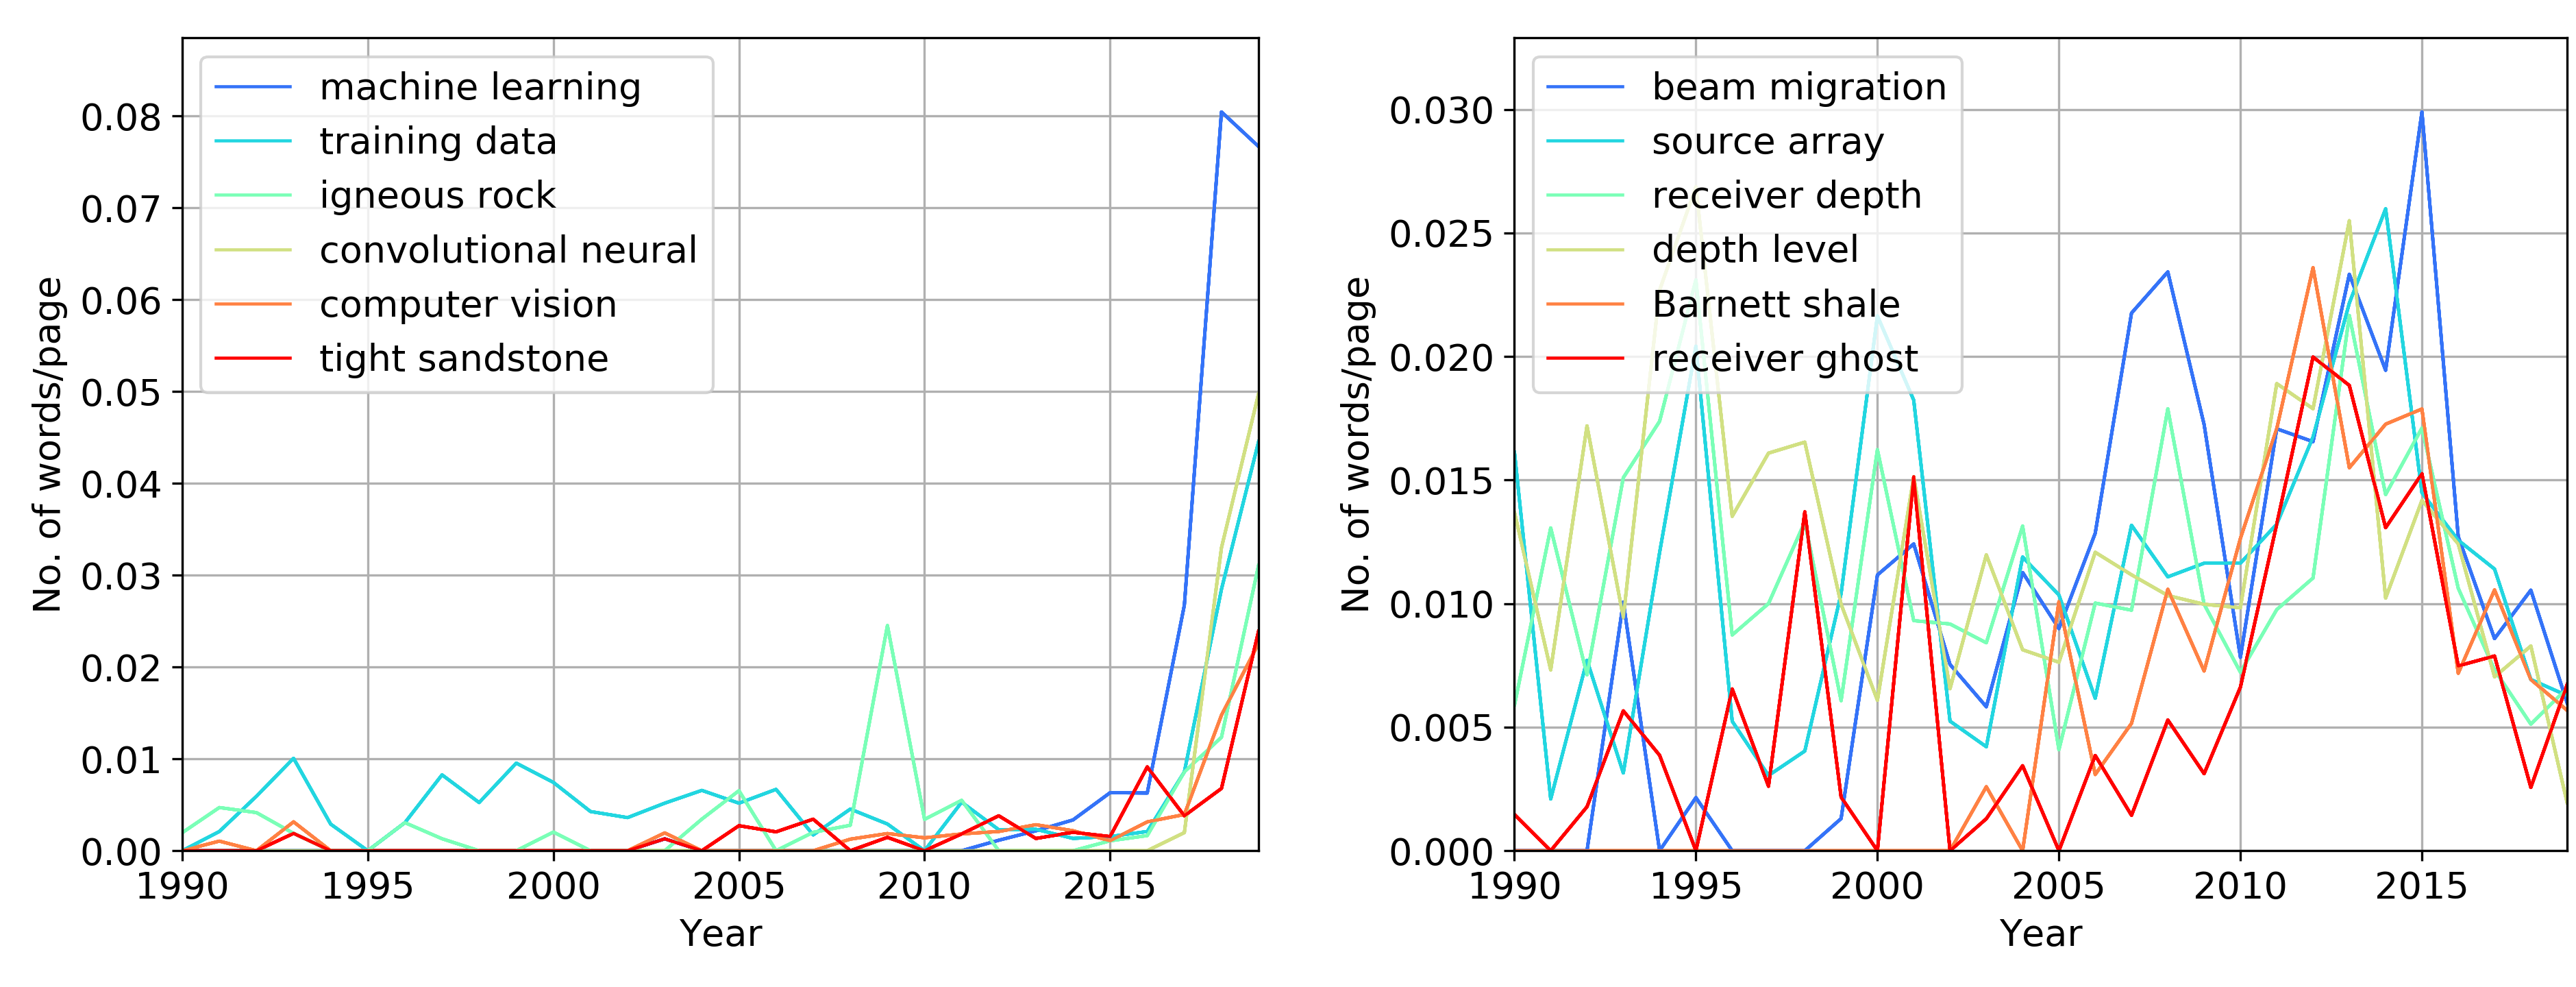
\includegraphics[width=\textwidth]{bi_grow_decl.png}}
\caption{Two-word phrases that show the highest rate of growth in occurrence (left) and decline (right) in the past four years.}
\label{bigrams}
\end{figure}


\begin{figure}[ht!]

\center{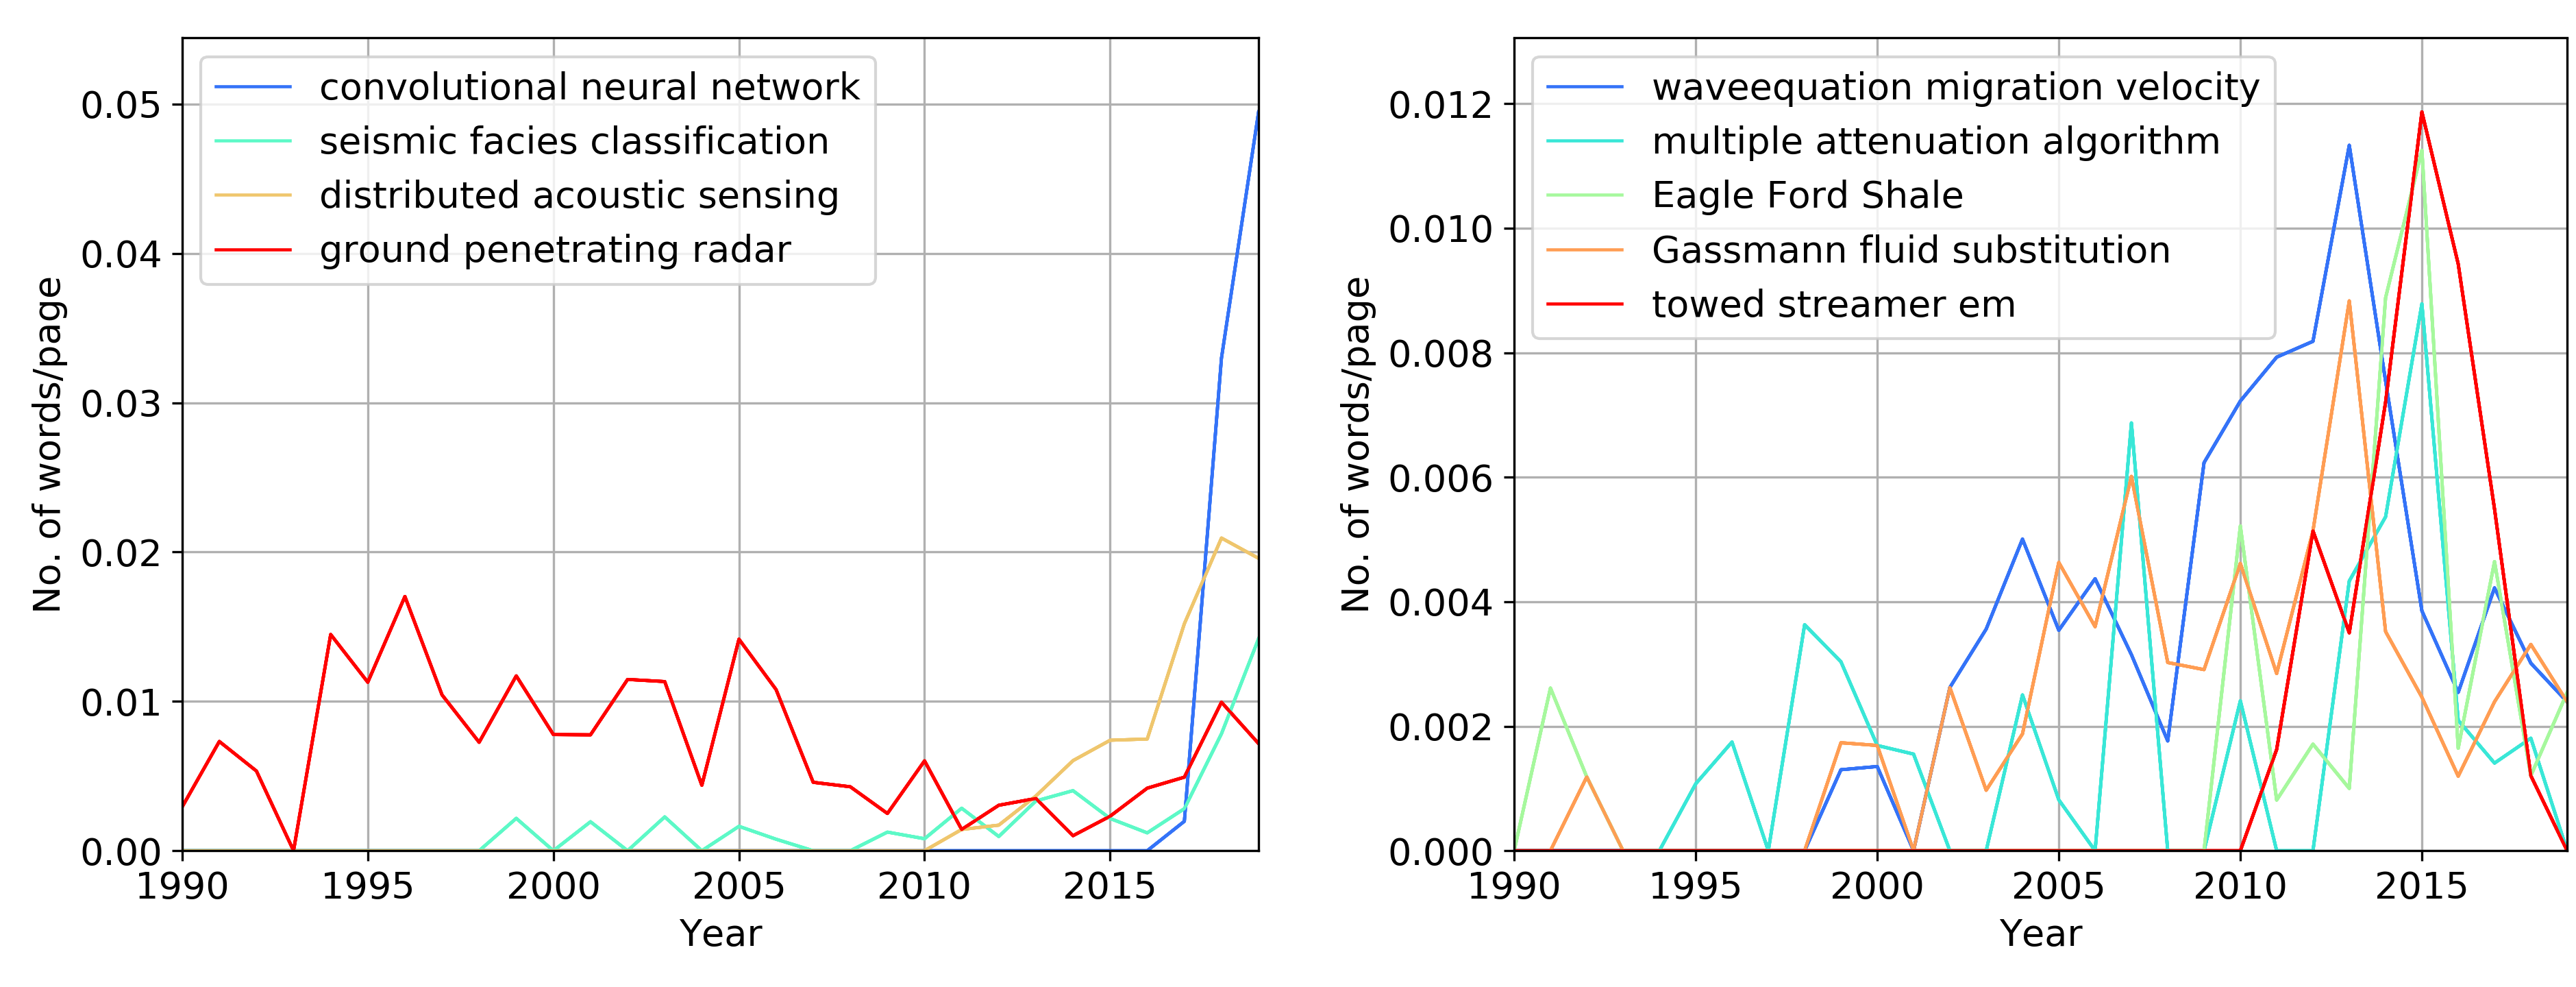
\includegraphics[width=\textwidth]{tri_grow_decl.png}}

\caption{Three-word phrases that show the highest rate of growth in occurrence (left) and decline (right) in the past four years.}
\label{trigrams}
\end{figure}

Let us consider the fastest growing and declining three-word phrases, Fig. \ref{trigrams}. ``Convolutional neural network'' (CNN) shows the fastest growth; the second one is ``distributed acoustic sensing'' (DAS), which is related to the fiber-optic measurement system. In the recent few years, researchers are using CNN to perform ``seismic facies classification,'' which is why we observe an increase in usage. We also see a relative increase for ``ground penetration radar,'' however, we see this term more often during the 1990s and early 2000. The right graph of Fig. \ref{trigrams} shows a decrease in the use of specific seismic terms as for the case of two-word phrases and the names of the shale deposits. From 2010 to 2019, we observe an increase and decrease in interest in the phrase ``towed streamer EM.'' Towed streamer electromagnetic systems allow one to collect data at a high rate and over huge survey areas \citep{Zhdanov2015}. It is necessary to have significant objects to survey broad areas. Nowadays, there are less large-scale oil exploration projects, so the researchers use the corresponding terms less often.

It would be interesting to trace how the different methods are developing in geophysics, electrical exploration methods, petrophysics, engineering geophysics. For this reason, it is worthwhile to study the materials of conferences and publications of other journals with a different specialization. Research on conference materials of other societies (SPWLA, EAGE, SPE) wwill provide a complete picture of the advances in the oil industry.

We encourage readers to use our data available online \citep{Eltsov2020}. The data includes the filtered word lists with the frequency of use each year, the number of pages, and the average number of co-authors. Thus, the reader will be able to conduct their research, test their hypotheses or assumptions.


%%%%%%%%%%%%%%%%%%%%%%%%%%%%%%%%%%%%%%%%%%
\section{Conclusions}

We analyzed 24,500 papers, including 127,900 pages consisting of 57 million words, or more than 383 million symbols. Alteration in the professional language reflects the change in the industry and science. Over the 30 years, the objects and geophysical methods changed slightly. There has been an increased interest in ``shales'' in the last ten years. In the past six years, the frequency of the use of the word ``shale'' has been falling, but the use of the phrases ``unconventional,'' ``TOS,'' ``hydraulic fracturing'' has not decreased in recent years. At the same time, new methods of processing and capturing data appeared, and this led to a change in language. "Neural network'' and related disciplines show the fastest growth in the last two years. The authors doubt that growth will continue at the same rate as the term ``neural network'' is already used more than ``field data.'' More likely, ``neural network'' related topics will occupy its niche in geophysics for the coming years. We see an increase in the use of the words ``Marchenko,'' ``seismicity,'' and ``broadband.'' We also observe the rapid growth of the word ``fiber,'' which is more likely related to fiber optic sensing systems. Supposedly, we will see more projects on ``monitoring'' of oil and gas fields and increasing production ``efficiency,'' while there will be less work on the exploration of new oil and gas fields.
 

%%%%%%%%%%%%%%%%%%%%%%%%%%%%%%%%%%%%%%%%%%
\vspace{6pt} 

%%%%%%%%%%%%%%%%%%%%%%%%%%%%%%%%%%%%%%%%%%
\authorcontributions{Data mining and processing, software development, original draft preparation - Timofey Eltsov; software development and analysis, review and editing of the draft - Maxim Yutkin; supervision, project administration, historical analysis, review, and editing of the paper - Tadeusz W. Patzek.}

%%%%%%%%%%%%%%%%%%%%%%%%%%%%%%%%%%%%%%%%%%
\funding{Dr. Eltsov was supported by the KAUST Magnetic Sensor project, REP-2708.}

%%%%%%%%%%%%%%%%%%%%%%%%%%%%%%%%%%%%%%%%%%
\acknowledgments{Authors appreciate the responsiveness of the SEG team for permission to use digital data and especially SEG Digital Publications Manager, Jeno Mavzer, for the useful advice and help. The authors are grateful to their colleagues, and especially to Dr. Thomas Finkbeiner, for valuable and vital research recommendations. The authors thank Dr. Sergey Yaskevich for consultations on exploration seismic. The authors are grateful to Ilya Kolganov for the useful advice on the design of the graphs. We also would like to acknowledge Dr. Charles Russell Severance for an informative Python course.}

%%%%%%%%%%%%%%%%%%%%%%%%%%%%%%%%%%%%%%%%%%
\conflictsofinterest{The authors declare no conflict of interest.} 

%%%%%%%%%%%%%%%%%%%%%%%%%%%%%%%%%%%%%%%%%%
%% optional
\abbreviations{The following abbreviations are used in this manuscript:\\

\noindent 
\begin{tabular}{@{}ll}
ASCII & American standard code for information interchange\\
AVO & Amplitude Variation with Offset\\
CNN & Convolutional Neural Network\\
CMP & Common Mid Point\\
CSEM & The Controlled Source Electromagnetic\\
DAS & Distributed Acoustic Sensing\\
EAGE & European Association of Geoscientists and Engineers\\
EM & Electromagnetic\\
FWI & Full Waveform Inversion\\
GPU & Graphics Processing Unit\\
HTML & HyperText Markup Language\\
NLTK & Natural Language Toolkit\\
NMO & Normal Moveout\\
PDF & Portable Document Format \\
PIL & Python Imaging Library\\
PSDM & Prestack Depth Migration\\
RTM & Reverse Time Migration\\
R\&D & Research and Development\\
SEG & Society of Exploration Geophysicists\\
SPE & Society of Petroleum Engineers\\
SPWLA & Society of Petrophysicists and Well Log Analysts \\
TXT & Text file\\
TOC & Total Organic Carbon\\
USA & The United States of America
\end{tabular}}
%%%%%%%%%%%%%%%%%%%%%%%%%%%%%%%%%%%%%%%%%%
%% optional
\appendixtitles{no} %Leave argument "no" if all appendix headings stay EMPTY (then no dot is printed after "Appendix A"). If the appendix sections contain a heading then change the argument to "yes".
\appendix

%\unskip
%\subsection{}
%The appendix is an optional section that can contain details and data supplemental to the main text. For example, explanations of experimental details that would disrupt the flow of the main text, but nonetheless remain crucial to understanding and reproducing the research shown; figures of replicates for experiments of which representative data is shown in the main text can be added here if brief, or as Supplementary data. Mathematical proofs of results not central to the paper can be added as an appendix.
%%
%\section{}
%All appendix sections must be cited in the main text. In the appendixes, Figures, Tables, etc. should be labeled starting with `A', e.g., Figure A1, Figure A2, etc. 

%%%%%%%%%%%%%%%%%%%%%%%%%%%%%%%%%%%%%%%%%%
\reftitle{References}

% Please provide either the correct journal abbreviation (e.g. according to the "List of Title Word Abbreviations" http://www.issn.org/services/online-services/access-to-the-ltwa/) or the full name of the journal.
% Citations and References in Supplementary files are permitted provided that they also appear in the reference list here. 

%=====================================
% References, variant A: external bibliography
%=====================================
%\externalbibliography{yes}
%\bibliography{your_external_BibTeX_file}
%\bibliography{timaref}
%=====================================
% References, variant B: internal bibliography
%=====================================
\begin{thebibliography}{999}
\providecommand{\natexlab}[1]{#1}

\bibitem[Glauner \em{et~al.}(2018)Glauner, Valtchev, and State]{Glauner2018}
Glauner, P.; Valtchev, P.; State, R.
\newblock {Impact of Biases in Big Data}.
\newblock In~Proceedings of the European Symposium on Artificial Neural Networks, Computational Intelligence and Machine Learning, Bruges, Belgium, 25-27 April~2018; pp 645--654.

\bibitem[Kaplan \em{et~al.}(2014)Kaplan, Chambers, and Glasgow]{Kaplan2014}
Kaplan, R.; Chambers, D.A.; Glasgow, R.E.
\newblock {Big Data and Large Sample Size: A Cautionary Note on the Potential for Bias}.
\newblock {\em CTS Journal} {\bf 2014}, {\em 7}, {4}, ~342--346.
\newblock
 doi:{\changeurlcolor{black}\href{ https://doi.org/10.1111/cts.12178}{\detokenize{10.1111/cts.12178}}}.

\bibitem[SEG, (2019)]{SEG}
\newblock {SEG Technical Program Expanded Abstracts. Available online: https://library.seg.org/series/segeab (Accessed on 2 December 2019)}.


\bibitem[Eltsov (2020)]{Eltsov2020}
Eltsov, T.
\newblock {Data for SEG Annual Conferences analysis, 1982 - 2019. Available online: https://github.com/ANPERC-source/SEG\_Annual (Accessed on 2 February 2020)}.


\bibitem[Mallapaty (2018)]{Mallapaty2018}
\newblock {Paper authorship goes hyper. Available online: https://www.natureindex.com/news-blog/paper-authorship-\\goes-hyper (Accessed on 17 October 2019)}.


\bibitem[Kroode \em{et~al.}(2014)]{Kroode2013}
Kroode, F.; Bergler, S.; Corsten, C.; Maag, J.W.D.; Strijbos, F.; Tijhof, H.
\newblock {Broadband seismic data — The importance of low frequencies}.
\newblock {\em Geophysics} {\bf 2013}, {\em 78}, {2}, ~WA3--WA14.
\newblock
 doi:{\changeurlcolor{black}\href{ https://doi.org/10.1190/GEO2012-0294.1}{\detokenize{10.1190/GEO2012-0294.1}}}.

\bibitem[Lomas and Curtis(2014)]{Lomas2019}
Lomas, A.; Curtis, A.
\newblock {An introduction to Marchenko methods for imaging}.
\newblock {\em Geophysics} {\bf 2019}, {\em 84}, {2}, ~35--45.
\newblock
 doi:{\changeurlcolor{black}\href{ https://doi.org/10.1190/geo2018-0068.1}{\detokenize{10.1190/geo2018-0068.1}}}.

\bibitem[Thorbecke \em{et~al.}(2017)]{Thorbecke2017}
Thorbecke, J.; Slob, E.; Brackenhoff, J.; Neut, J.V.D.; Wapenaar, K.
\newblock {Implementation of the Marchenko method}.
\newblock {\em Geophysics} {\bf 2017}, {\em 82}, {6}, ~WB29--WB45.
 doi:{\changeurlcolor{black}\href{https://doi.org/10.1190/geo2017-0108.1}{\detokenize{10.1190/geo2017-0108.1}}}

\bibitem[Iervolino \em{et~al.}(2016)]{Iervolino2016}
Iervolino, I.; Giorgio, M.; Chioccarelli, E.
\newblock {Markovian modeling of seismic damage accumulation}.
\newblock {\em Earthquake Engineering {\&} Structural Dynamics} {\bf 2016}, {\em 45}, {November 2015}, ~441--461.
\newblock
 doi:{\changeurlcolor{black}\href{ https://doi.org/10.1002/eqe}{\detokenize{10.1002/eqe}}}.

\bibitem[Weir \em{et~al.}(2018)]{Weir2018}
Weir, R.; Lines, L.; Lawton, D.; Eyre, T.
\newblock {The Duvernay Formation : the application of structure and simultaneous inversion for reservoir characterization and induced seismicity}.
\newblock In~Proceedings of the SEG Annual Conference and Exhibition, Anaheim, USA, 14-19 October~2018; pp 2372--2376.
doi:{\changeurlcolor{black}\href{ https://doi.org/10.1190/segam2018-2980345.1}{\detokenize{10.1190/segam2018-2980345.1}}}.

\bibitem[Barthwal and Baan(2018)]{Barthwal2018}
Barthwal, H.; Baan, M.V.D.
\newblock {Causative mechanism of microseismicity recorded in an underground mine}.
\newblock In~Proceedings of the SEG Annual Conference and Exhibition, Anaheim, USA, 14-19 October~2018; pp 2962--2966.
doi:{\changeurlcolor{black}\href{ https://doi.org/10.1190/segam2018-2980345.1}{\detokenize{10.1190/segam2018-2980345.1}}}.

\bibitem[Trainor-Guitton \em{et~al.}(2018)Trainor-Guitton, Jreij, Guitton, and Simmons]{Trainor-Guitton2018}
Trainor-Guitton, W.; Jreij, S.; Guitton, A.; Simmons, J. 
\newblock {Fault classification from 3D imaging of vertical DAS profile}.
\newblock In~Proceedings of the SEG Annual Conference and Exhibition, Anaheim, USA, 14-17 October~2018; pp 4664--4668.

\bibitem[Binder and Chakraborty(2018)]{Binder2019}
Chakraborty, G.; Chakraborty, D. 
\newblock {Detecting microseismic events in downhole distributed acoustic sensing data using convolutional neural networks}.
\newblock In~Proceedings of the SEG Annual Conference and Exhibition, San Antonio, USA, 15-20 September~2019; pp 4864--4868.



\bibitem[Penna \em{et~al.}(2019)Penna, Ara{\'{u}}jo, Geisslinger, Sansonowski, Oliveira, Rosseto, and Matos]{Penna2019}
Penna, R.; Ara{\'{u}}jo, S.; Geisslinger, A.; Sansonowski R.; Oliveira, L.; Rosseto J.; Matos, M.
\newblock {Carbonate and igneous rock characterization through reprocessing, FWI imaging, and elastic inversion of a legacy seismic data set in Brazilian presalt province}.
\newblock {\em The Leading Edge} {\bf 2019}, {\em 38}, {1}, ~11--19.
\newblock
 doi:{\changeurlcolor{black}\href{ https://doi.org/10.1190/tle38010011.1}{\detokenize{10.1190/tle38010011.1}}}.

\bibitem[Merriam-Webster(2020)]{MW2020}
Merriam-Webster online dictionary.
\newblock {Available online: https://www.merriam-webster.com/ (Accessed on 16 February 2020)}.


\bibitem[Hill(1990)]{Hill1990}
Hill, N.R.;
\newblock {Gaussian beam migration}.
\newblock {\em Geophysics} {\bf 1990}, {\em 55}, {11}, ~1416--1428.
 doi:{\changeurlcolor{black}\href{https://doi.org/10.1190/1.1442788}{\detokenize{10.1190/1.1442788}}}

\bibitem[Huang \em{et~al.}(2001)Huang, Sherrill, and Sengupta]{Huang2001}
Huang, S.; Sherrill, F.; Sengupta, M.K. 
\newblock {Merits of amplitude preserving Kirchhoff beam migration method for 3D AVO analysis}.
\newblock In~Proceedings of the SEG Annual Conference and Exhibition, San Antonio, USA, 9-14 September~2001; pp 1--4.

\bibitem[Ting and Wang(2008)]{Ting2008}
Ting, C.O.; Wang, D.
\newblock {Controlled beam migration applications in Gulf of Mexico}.
\newblock In~Proceedings of the SEG Annual Conference and Exhibition, Las Vegas, USA, 9-14 November~2008; pp 368--372.

\bibitem[Zhdanov \em{et~al.}(2001)Zhdanov, Endo, Sunwall, and Mattsson]{Zhdanov2015}
Zhdanov, M.S.; Endo, M.; Sunwall, D.; Mattsson, J.
\newblock {Advanced 3D imaging of complex geoelectrical structures using towed streamer EM data}.
\newblock In~Proceedings of the SEG Annual Conference and Exhibition, New Orleans, USA, 18-23 October~2015; pp 904--908.


\end{thebibliography}
%%%%%%%%%%%%%%%%%%%%%%%%%%%%%%%%%%%%%%%%%%
%% optional
%\sampleavailability{Samples of the compounds ...... are available from the authors.}

%% for journal Sci
%\reviewreports{\\
%Reviewer 1 comments and authors’ response\\
%Reviewer 2 comments and authors’ response\\
%Reviewer 3 comments and authors’ response
%}

%%%%%%%%%%%%%%%%%%%%%%%%%%%%%%%%%%%%%%%%%%
\end{document}


%%% Local Variables:
%%% mode: latex
%%% TeX-master: t
%%% End:
